\section{Roboterbau}

In diesem Teil werden die einzelnen Schritte beschrieben, um den Roboter zu bauen. Dabei wird sich an dem Konzept von \acrshort{pren1} orientiert. Falls von dem Konzept abgewichen wird, wird dies erwähnt und begründet.

Die folgenden Kapitel sind unterteilt nach den einzelnen Funktionen des Roboters. Dabei werden die Tätigkeiten beschrieben, inklusive Testprotokolle und -beschriebe.

TODO: Risikoverweise (welches Risiko vermindert/behoben? \\
TODO: Testprotokolle \\
TODO: Lessons Learned \\
TODO: Komponentendiagramme mit Schnittstellen falls sinnvoll \\

\subsection{Produktbeschreibung}

In diesem Kapitel wird der Roboter als Gesamtsystem beschrieben. Dabei wird das Funktionsmuster mit einem Ablaufdiagramm beschrieben und die einzelnen physischen und elektronischen Komponenten werden in einer Zeichnung, respektive einem Blockdiagramm aufgezeigt.



Damit dieses Funktionsmuster umgesetzt werden kann, wird ein Produkt mit folgenden Komponenten auf Grafik \ref{fig:components} gebaut. Die Grafik ist zeigt lediglich das Konzept mit den nötigen Komponenten und nicht das tatsächliche Aussehen des Roboters.

\begin{figure}[H]
\centering
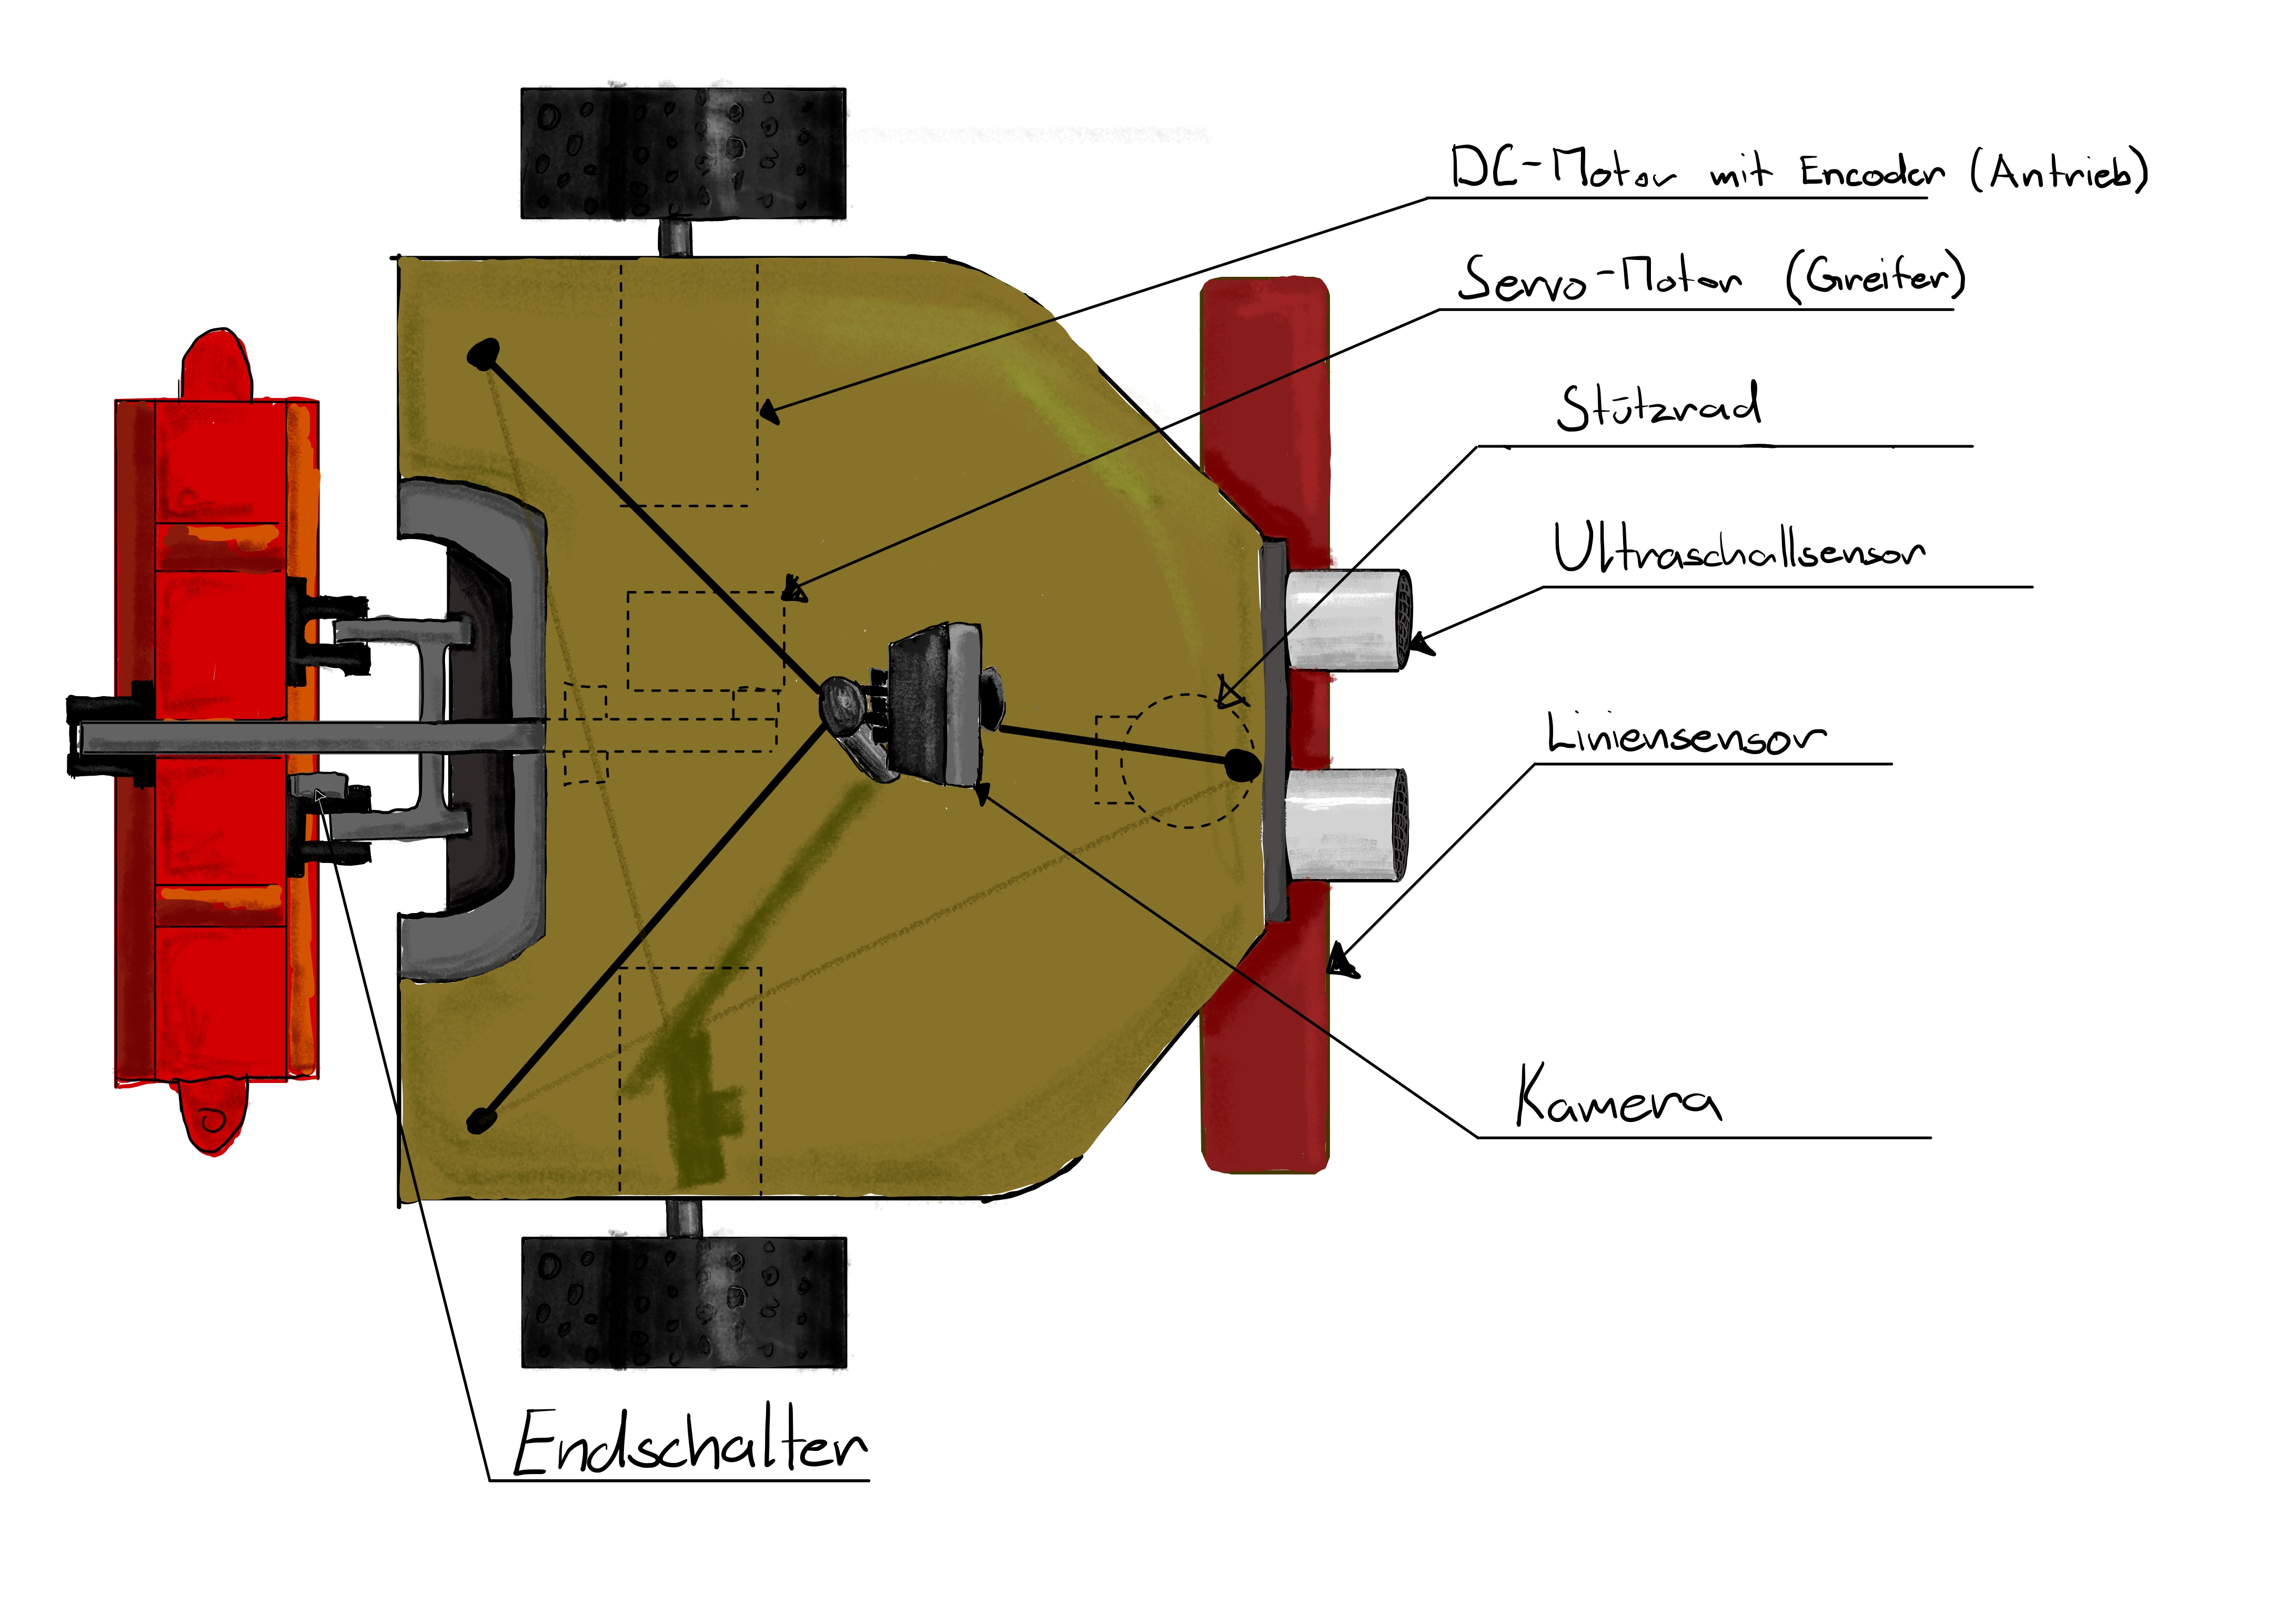
\includegraphics[width=\textwidth]{assets/gesamtkonzept/Skizze-Fahrzeugkonzept-Beschriftet.jpg}
\caption{Komponenten des Roboters}
\label{fig:components}
\end{figure}

Es wurde folgender Roboter gebaut, der die geplanten Komponenten enthält.
TODO BILD ROBOTER

Die folgende Grafik \ref{fig:ablauf} zeigt den geplanten Ablauf auf. Dieses Ablaufdiagramm stammt aus \acrshort{pren1} und dient zur Erinnerung, genauere Informationen können aus der angehängten PREN 1 Dokumentation entnommen werden.

\begin{figure}[H]
\centering
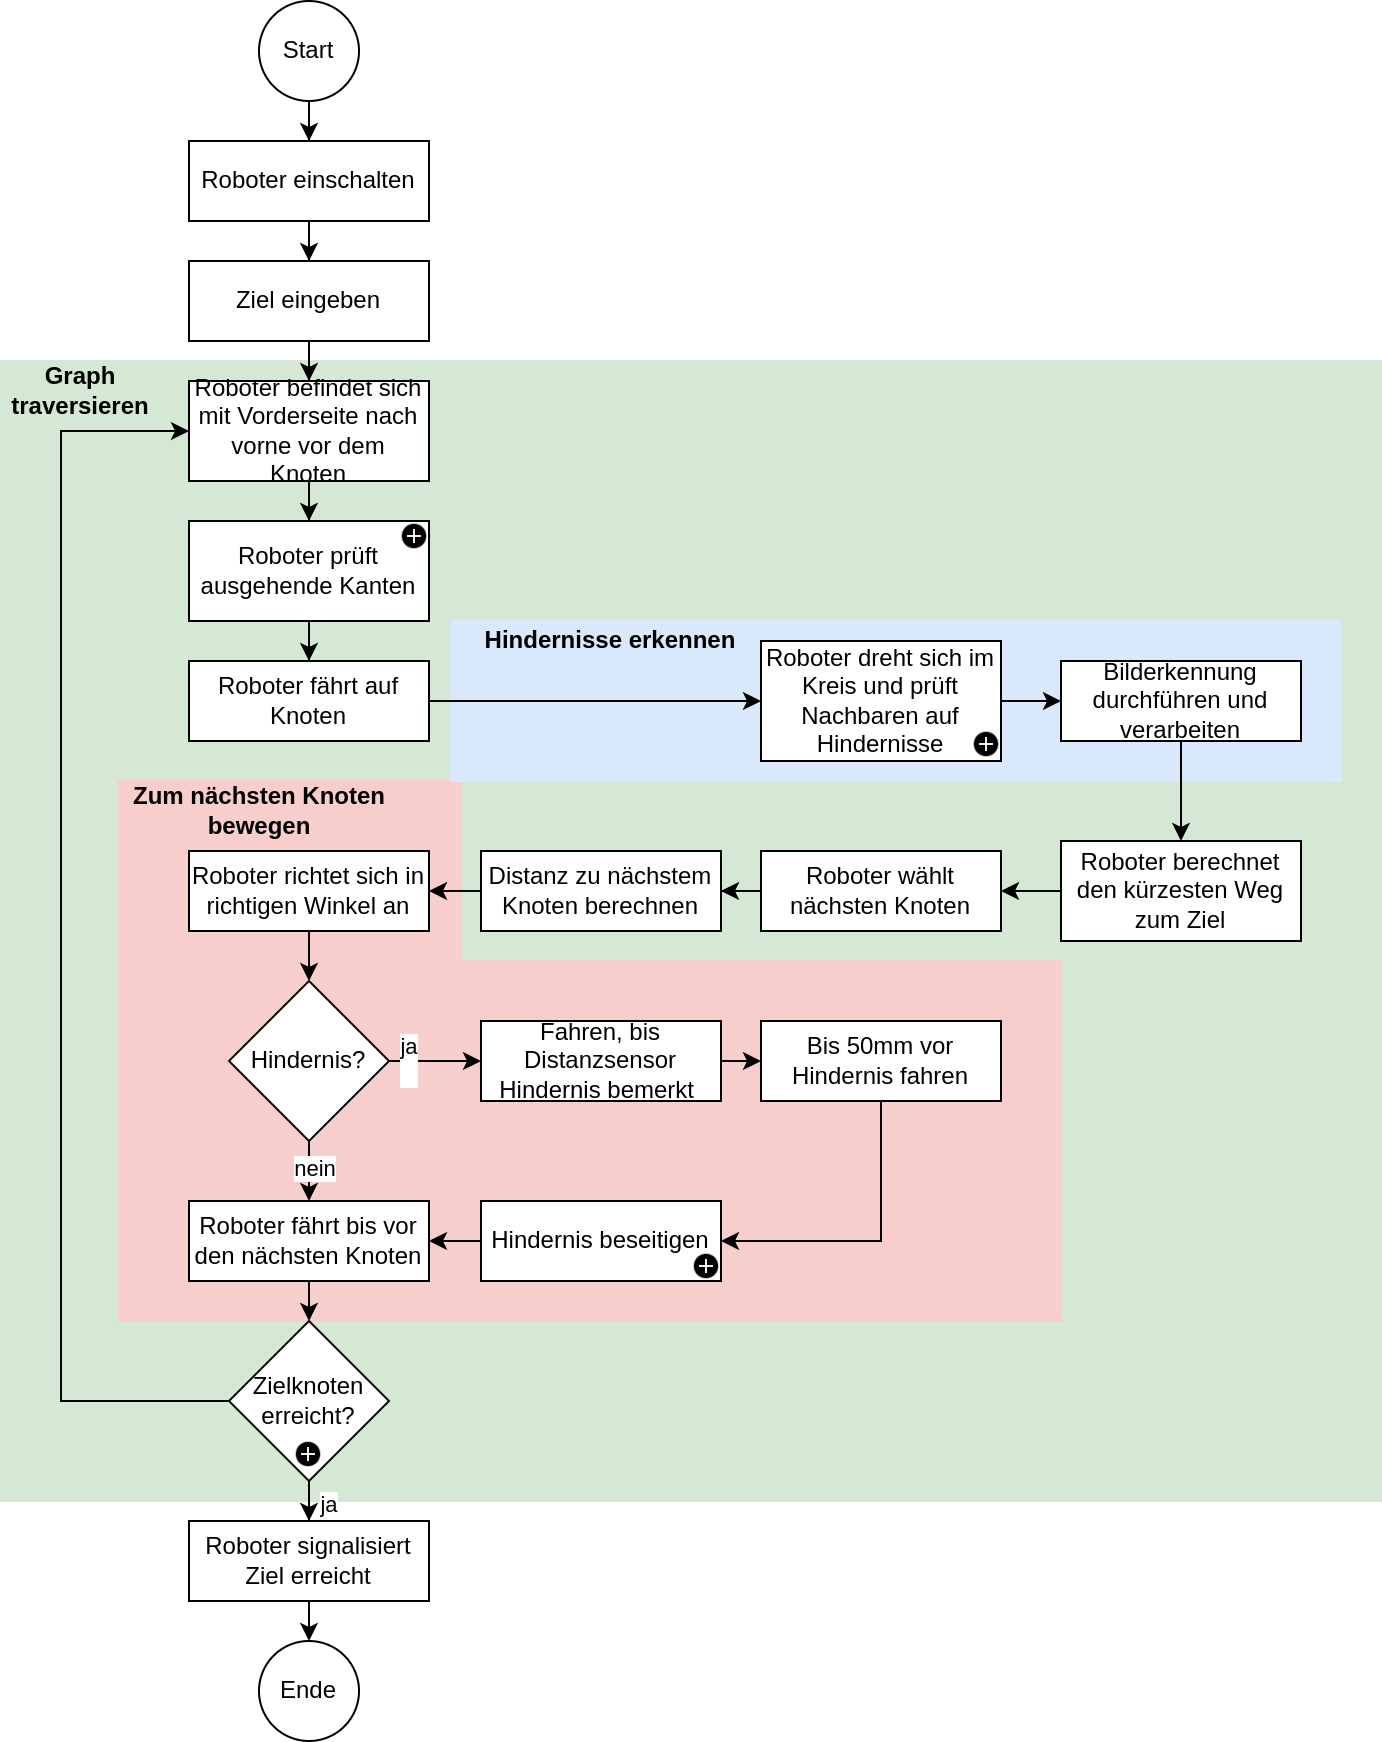
\includegraphics[width=\textwidth]{assets/gesamtkonzept/ablaufdiagramm.png}
\caption{Gesamtkonzept Ablaufdiagramm}
\label{fig:ablauf}
\end{figure}


Die einzelnen elektronischen Teile im Roboter bilden das Gesamtsystem ersichtlich auf Grafik \ref{fig:electro-components}. Dieses sorgt dafür, dass sich der Roboter wie geplant autonom fortbewegen kann.  Die Graphik ist aufgeteilt in die Teile, die Teil der Navigation sind und diese, die Teil der Steuerung sind. 

Das PCBA ist die zentrale Verbindung. Der TinyK22 liest den Ultraschall, Liniensensor, die Encoder und die Endschalter des Greifers aus und steuert den Servomotor und die Motorentreiber. Der Raspberry Pi und der TinyK22 kommunizieren über UART. Der Raspberry Pi steuert die Kamera an und liest den Startknopf und den Zielauswahlknopf an und zeigt auf dem Display das gewählte Ziel und die Zeit an, die seit dem Start vergangen ist.

TODO separate graphics to have nav/steuerung

\begin{figure}[H]
\centering
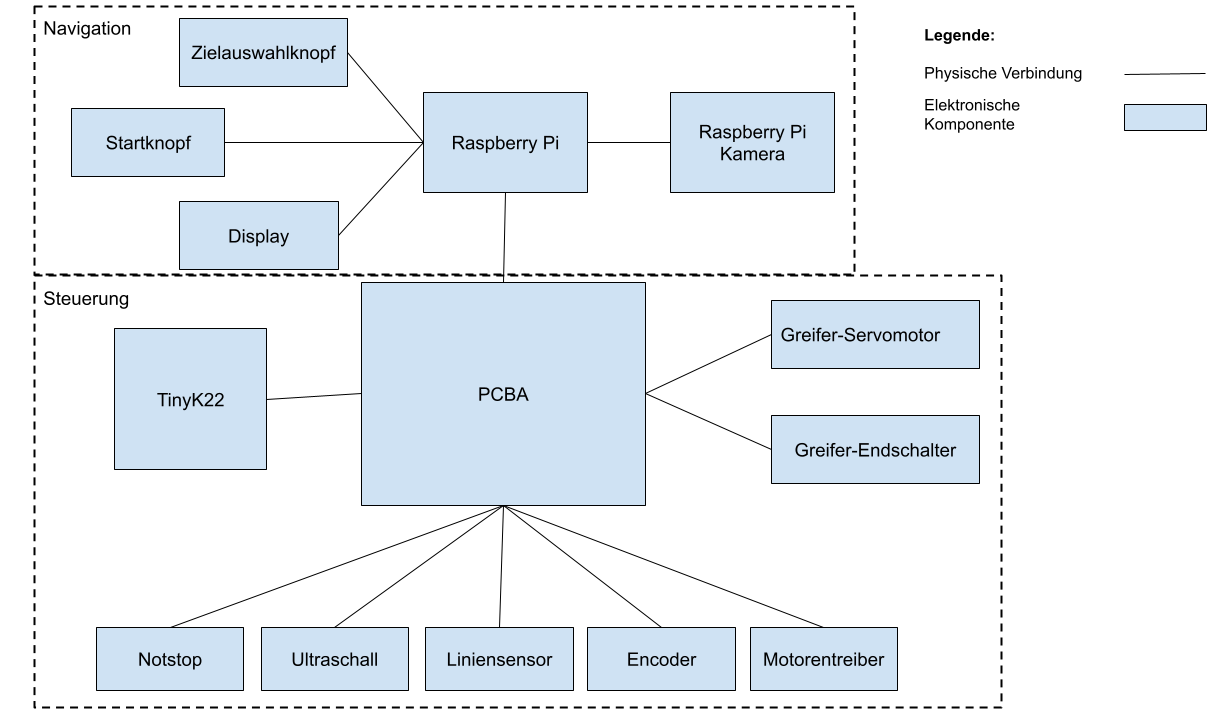
\includegraphics[width=\textwidth]{assets/gesamtkonzept/electronics.png}
\caption{Elektronische Komponenten des Roboters}
\label{fig:electro-components}
\end{figure} 

\newpage

\subsection{Mechanische Komponenten}
\label{Mechanische Komponenten}

Im nachfolgenden Kapitel wird auf die Konstruktion der mechanischen Komponenten eingegangen. Alle Konstruktionsbauteile, bis auf die Grundplatte, wurden im FDM-Verfahren aus PLA gedruckt. Zum Verschrauben der verschiedenen Bauteilen wurden M3 Gewindeeinsätze verwendet.

\subsubsection{Fahrwerk konstruieren}
\label{Fahrwerk konstruieren}

 Das Konzept für das Fahrwerk und die Grundplatte wurden analog zum Konzept aus \acrshort{pren1} umgesetzt. Am Fahrwerk wurden gegenüber des Prototyps aus \acrshort{pren1} einzig der Motorflansch und der Lenkrollenhalter angepasst. 
 Beim Prototyp in PREN 1 hat sich gezeigt, dass eine reine Presspassung für die Befestigung der Lenkrolle im Lenkrollenhalter aus PLA nicht ausreichend ist. Aus diesem Grund wird die Lenkrolle jetzt mithilfe eines M4 Gewindestifts geklemmt, wie gezeigt auf Abbildung \ref{fig: Lenkrollenhalter V2}.

\begin{figure}[H]
\centering
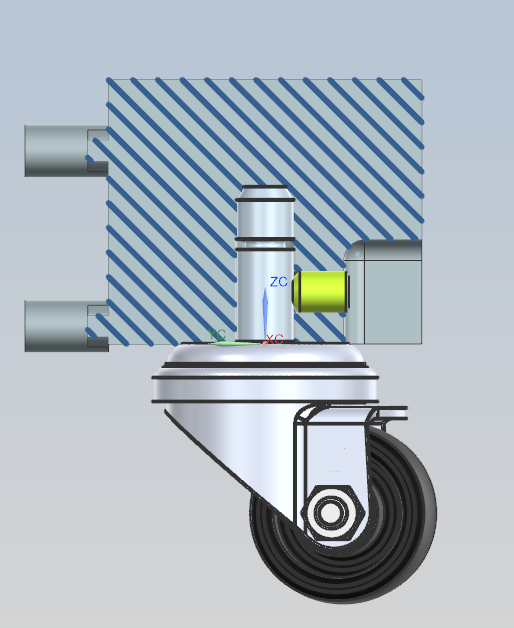
\includegraphics[width=5cm]{assets/MT/Lenkrollenhalter V2.png}
\caption{Lenkrollenhalter V2}
\label{fig: Lenkrollenhalter V2}
\end{figure}

Der Motorflansch wurde für den finalen Roboter leicht verstärkt. In Abbildung \ref{fig: Motorflansch V1/V2} sieht man in gelb die erste Version des Motorflansches wie er in PREN 1 verbaut wurde. Blau eingefärbt ist die finale Version des Flansches mit einer Verstrebung. 

\begin{figure}[H]
\centering
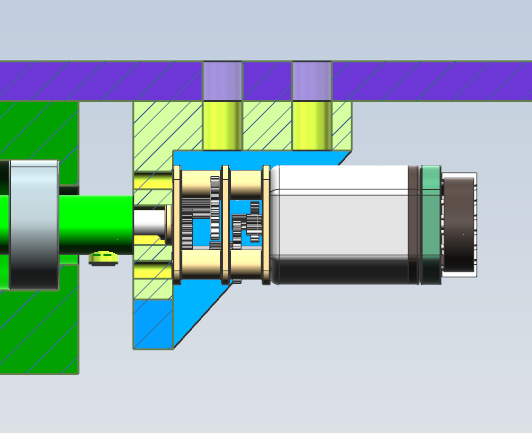
\includegraphics[width=5cm]{assets/MT/Motorflansch Vergleich.png}
\caption{Motorflansch V1/V2}
\label{fig: Motorflansch V1/V2}
\end{figure}

\subsubsection{Montage der Elektronischen Komponenten}
\label{Montage der Elektronischen Komponenten}

Die elektronischen Komponenten wie DC/DC-Konverter, Motortreiber oder Raspberry Pi werden nicht direkt auf die Grundplatte montiert, sondern auf Träger, welche anschliessend auf die Grundplatte geschraubt werden. Die Träger wurden so konstruiert, dass die Kabel zwischen Träger und Bauteilen geführt werden können. (siehe Abbildung \ref{fig: Träger für elektronische Komponenten}) Dieser Aufbau hatte in der frühen Testphase den Vorteil, dass alle elektronischen Komponenten provisorisch platziert werden konnten, ohne einen Kurzschluss zu riskieren. 

\begin{figure}[H]
\centering
\includegraphics[width=5cm]{assets/MT/Träger El Komponenten.jpg}
\caption{Träger für elektronische Komponenten werden zur Kabelführung verwendet}
\label{fig: Träger für elektronische Komponenten}
\end{figure}

\subsubsection{Batteriefach konstruieren}
\label{Batteriefach konstruieren}

Das Batteriefach wurde so konstruiert das sich die Batterie für die Lagerung jederzeit entfernen lässt. Dafür wurde ein Click-Verschluss verwendet. Das Batteriefach wird von unten in die Grundplatte geschoben bis es einrastet. Zum Herausnehmen der Batterie müssen nur die Haken gedrückt werden und das Batteriefach kann ausgefahren werden. Um die Funktion problemlos zu gewährleisten dürfen die Wandstärken nicht zu gross sein. Das die Festigkeit trotzdem gewährleistet werden kann wurde die Layerrichtung im 3D Drucker, wie in Abbildung \ref{Layerrichtung Batteriefach} so gewählt das die Layer horizontal zur Verschiebung der Hacken angeordnet sind. Auf Grund der Risikoanalyse in Tabelle \ref{table:risks} wurde entschieden als zusätzliche Vorsichtsmassnahme eine zweite Halterung herzustellen. So kann bei einem Defekt ohne Unterbruch weiter gearbeitet werden. \ref{table:risks}


\begin{figure}[H]
\centering
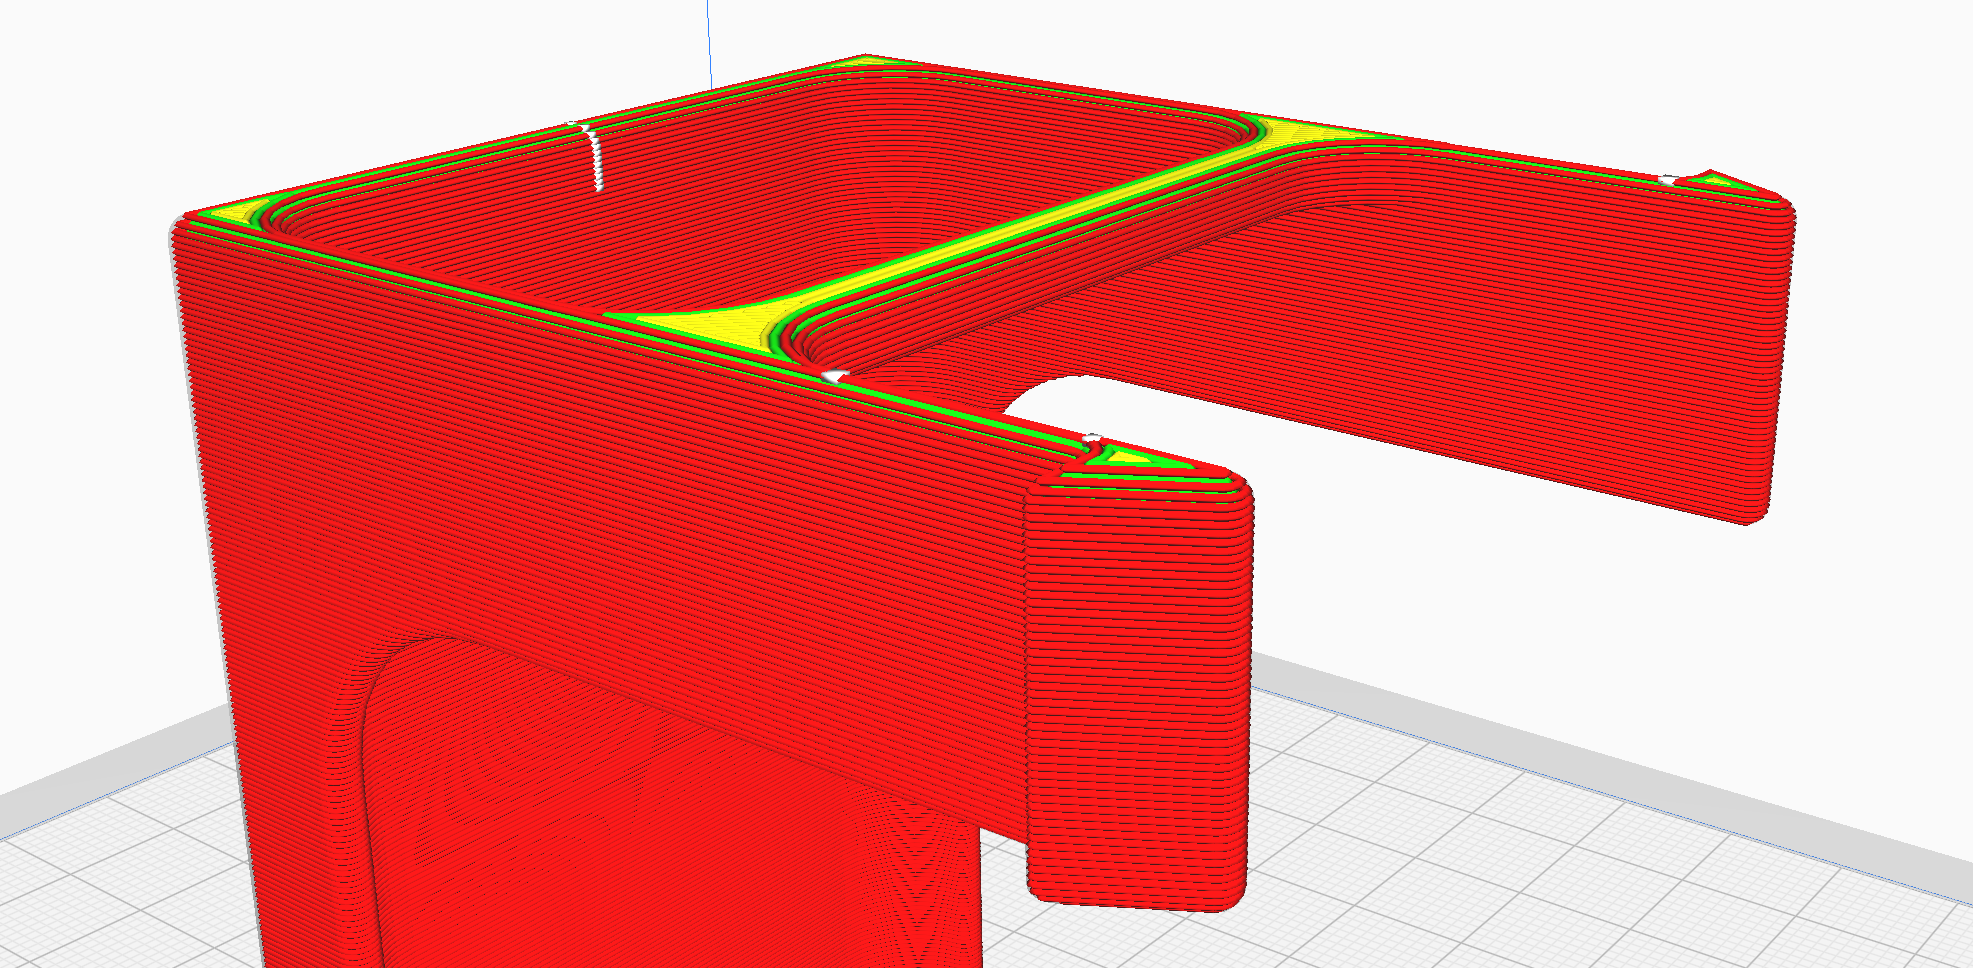
\includegraphics[width=\textwidth]{assets/MT/Layer_Batterie Fach.png}
\caption{Layerrichtung Batteriefach}
\label{Layerrichtung Batteriefach}
\end{figure}

\subsubsection{Greifer konstruieren}
\label{Greifer konstruieren}

Der Klemm- und Hebemechanismus des Greifers sind abhängig von der Federkraft und den Lagerstellen. Bei der Implementierung des Greifers musste darauf geachtet werden, dass die Lagerstellen nicht verschoben werden. In Abbildung \ref{fig:Greifer im Roboter} \& \ref{fig:Greifer Versuchsaufbau} sieht man die für die Funktion wichtigsten Masse am Versuchsaufbau und am fertigen Roboter. Die für die Haltekraft verantwortliche Feder, sowie alle Haltebacken und Pendelstützen wurden vom Prototyp wiederverwendet. 

\begin{figure}[H]
  \centering
  \begin{minipage}[b]{0.45\textwidth}
    \centering
    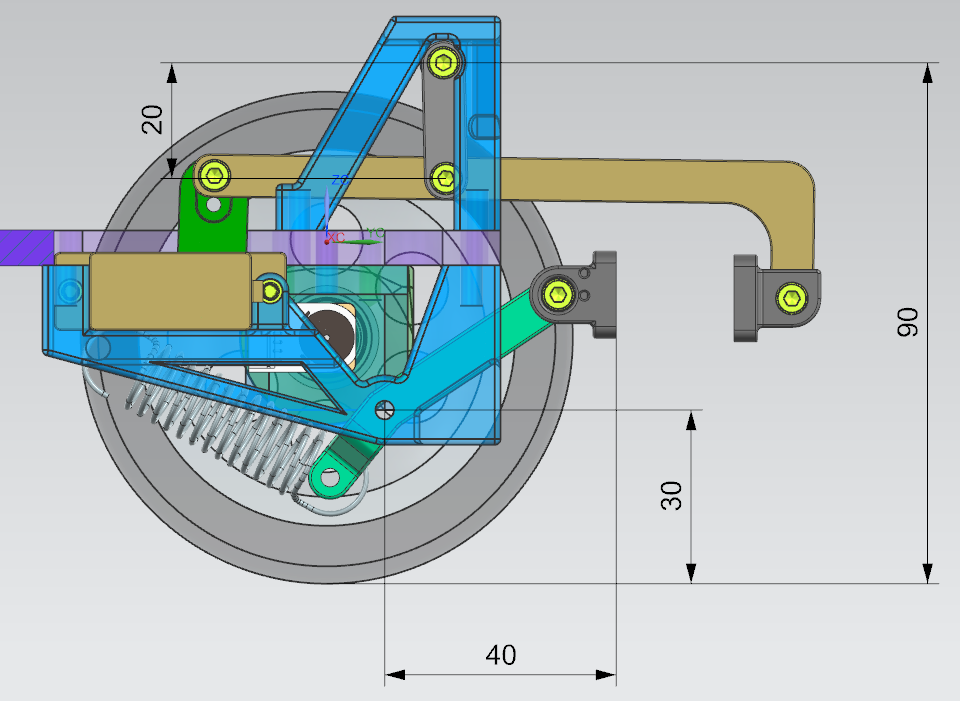
\includegraphics[height=5cm]{assets/MT/Greifer Montiert.png}
    \caption{Greifer im Roboter}
    \label{fig:Greifer im Roboter}
  \end{minipage}
  \hfill
  \begin{minipage}[b]{0.45\textwidth}
    \centering
    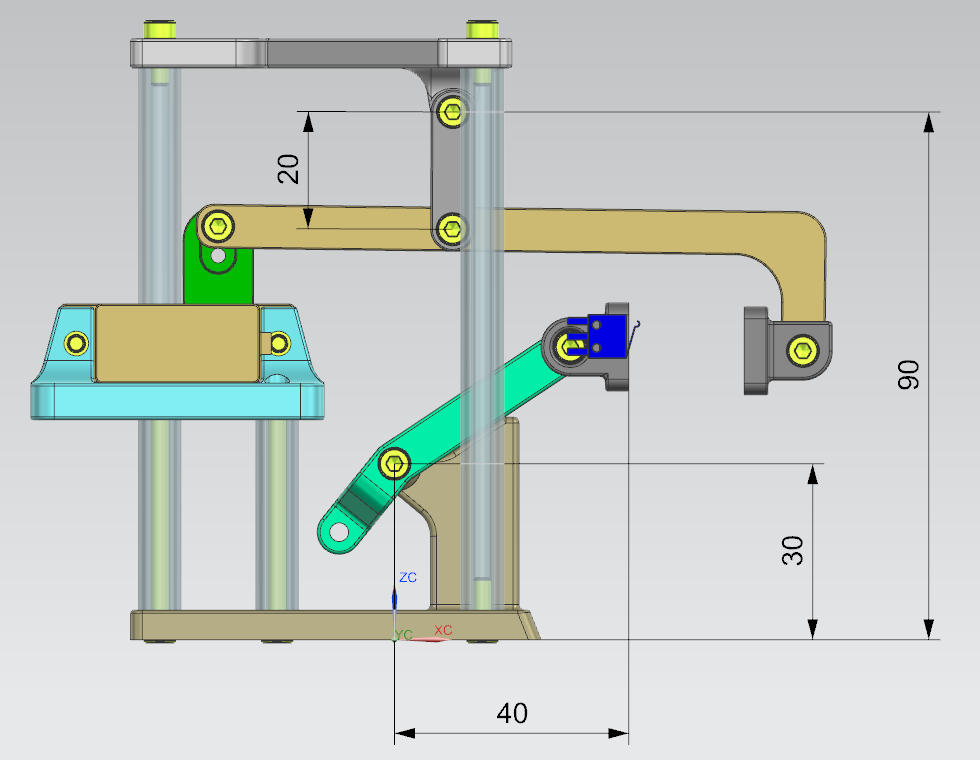
\includegraphics[height=5cm]{assets/MT/Greifer Prototyp.png}
    \caption{Greifer Versuchsaufbau}
    \label{fig:Greifer Versuchsaufbau}
  \end{minipage}
\end{figure}

\newpage

\subsubsection{Halterung Liniensensor}
\label{Halterung Liniensensor}

Der Liniensensor wird mit einer zweiteiligen Halterung befestigt. Auf der inneren Schale, in Abbildung \ref{fig:Schnitt Halterung Liniensensor} blau, ist der Sensor befestigt. Die innere Schale lässt sich verschieben. So kann die Höhe eingestellt werden. Die Fixierung erfolgt mithilfe von zwei Gewindestiften die in der äusseren Schale befestigt werden und die innere Schale klemmen. 


\begin{figure}[H]
    \centering
    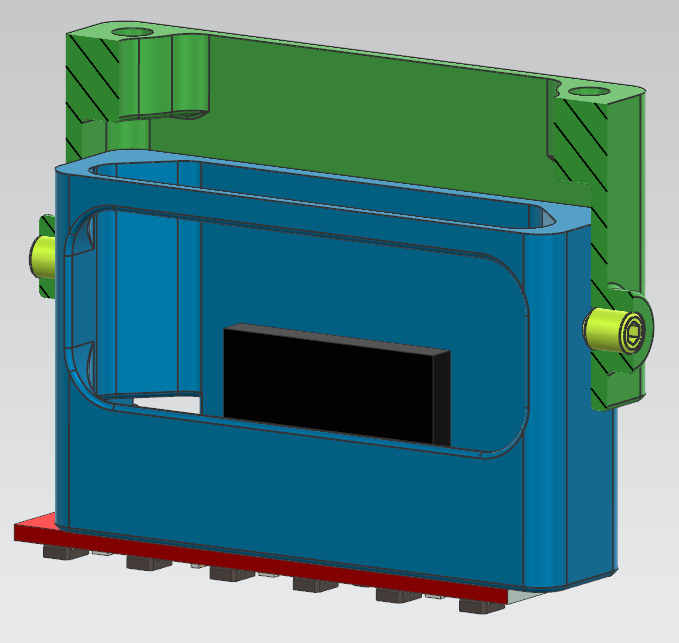
\includegraphics[width=0.75\linewidth]{assets//MT/Sensor Halterung.png}
    \caption{Schnitt Halterung Liniensensor}
    \label{fig:Schnitt Halterung Liniensensor}
\end{figure}


\subsubsection{Abschirmung des Liniensensors}
\label{Abschirmung des Liniensensors}

Um Störungen durch Fremdlicht zu verhindern wurde eine Abdeckung konstruiert, die jegliche Fremdeinstrahlung abschirmt. Als Dichtung wurde ein Bürstenband verwendet, wie es üblicherweise bei Schiebetüren zum Einsatz kommt. Die Bürsten werden in einer Halterung eingesteckt und mit einem Gewindestift geklemmt. 


\begin{figure}[H]
    \centering
    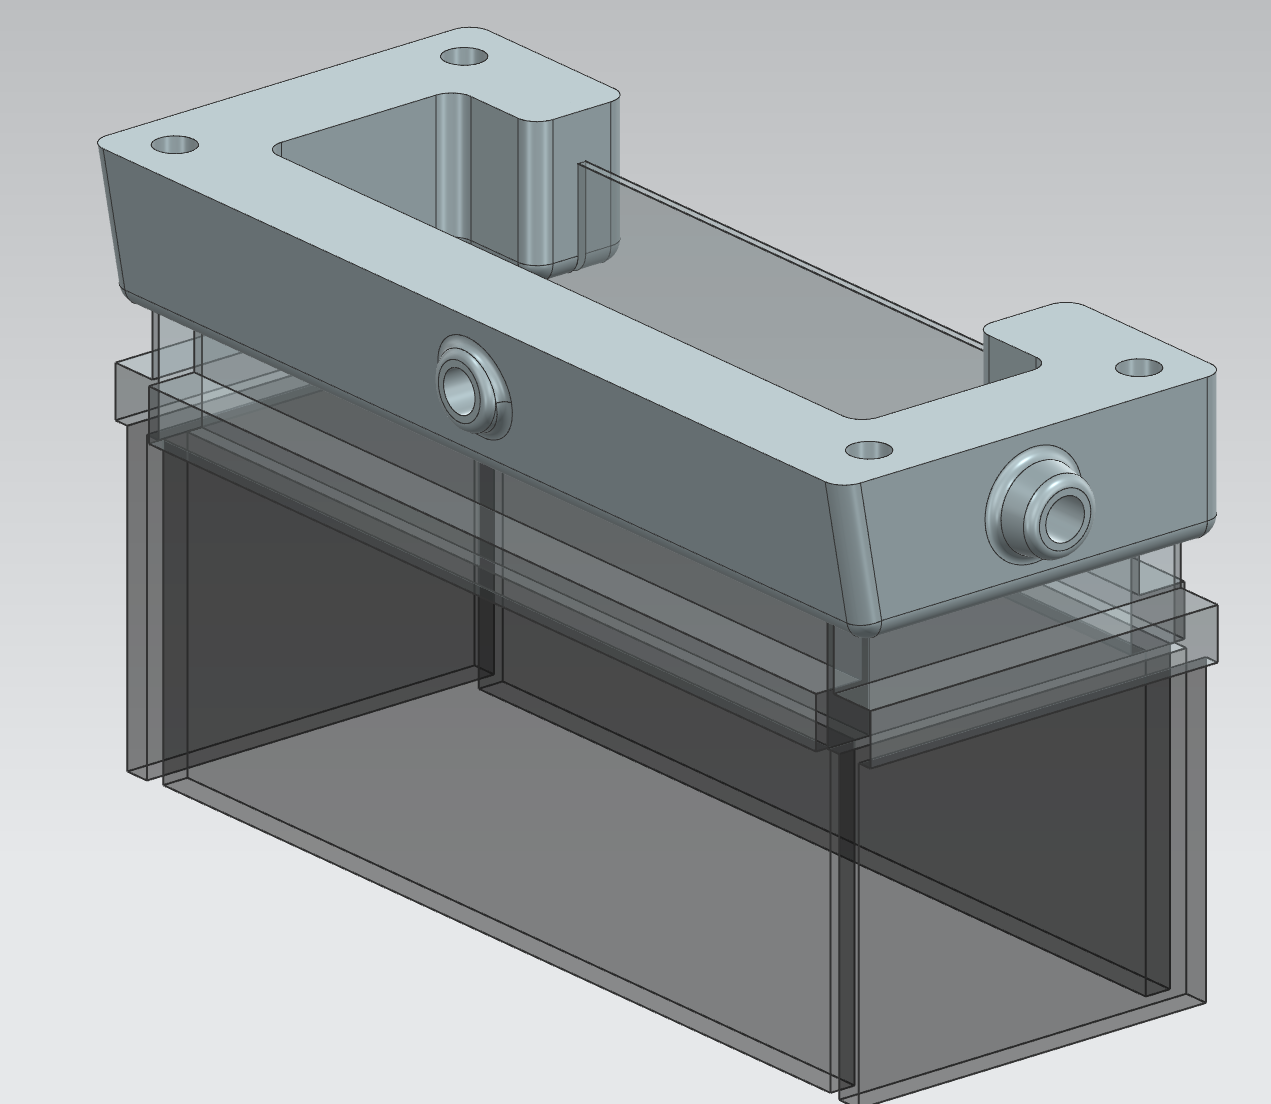
\includegraphics[width=0.75\linewidth]{assets//MT/Sensor Abdeckung.png}
    \caption{Liniensensor Abdeckung}
    \label{fig:Liniensensor Abdeckung}
\end{figure}
\newpage

\subsubsection{Ultraschall}

Es wird ein Ultraschallsensor montiert. Dieser wird gebraucht für die Bewältigung der Hindernisse und ebenfalls dient er als Backup, um Objekte zu erkennen. Falls die Kamera ein Objekte nicht erkennt, dann würde der Ultraschall dieses bemerken, wenn der Roboter sich davor befindet. Das sorgt dafür, dass Kollisionen vermieden werden.

Der Ultraschall wird ganz vorne am Roboter angebracht, auf der Höhe, die optimal ist, um die Barriere zu erkennen. Der Ultraschall misst direkt über den Löchern, die es in der Barriere gibt, so können die Wellen sicher an einer geraden Fläche reflektiert werden.

\begin{figure}[H]
\centering
\begin{minipage}[b]{0.45\textwidth}
  \centering
  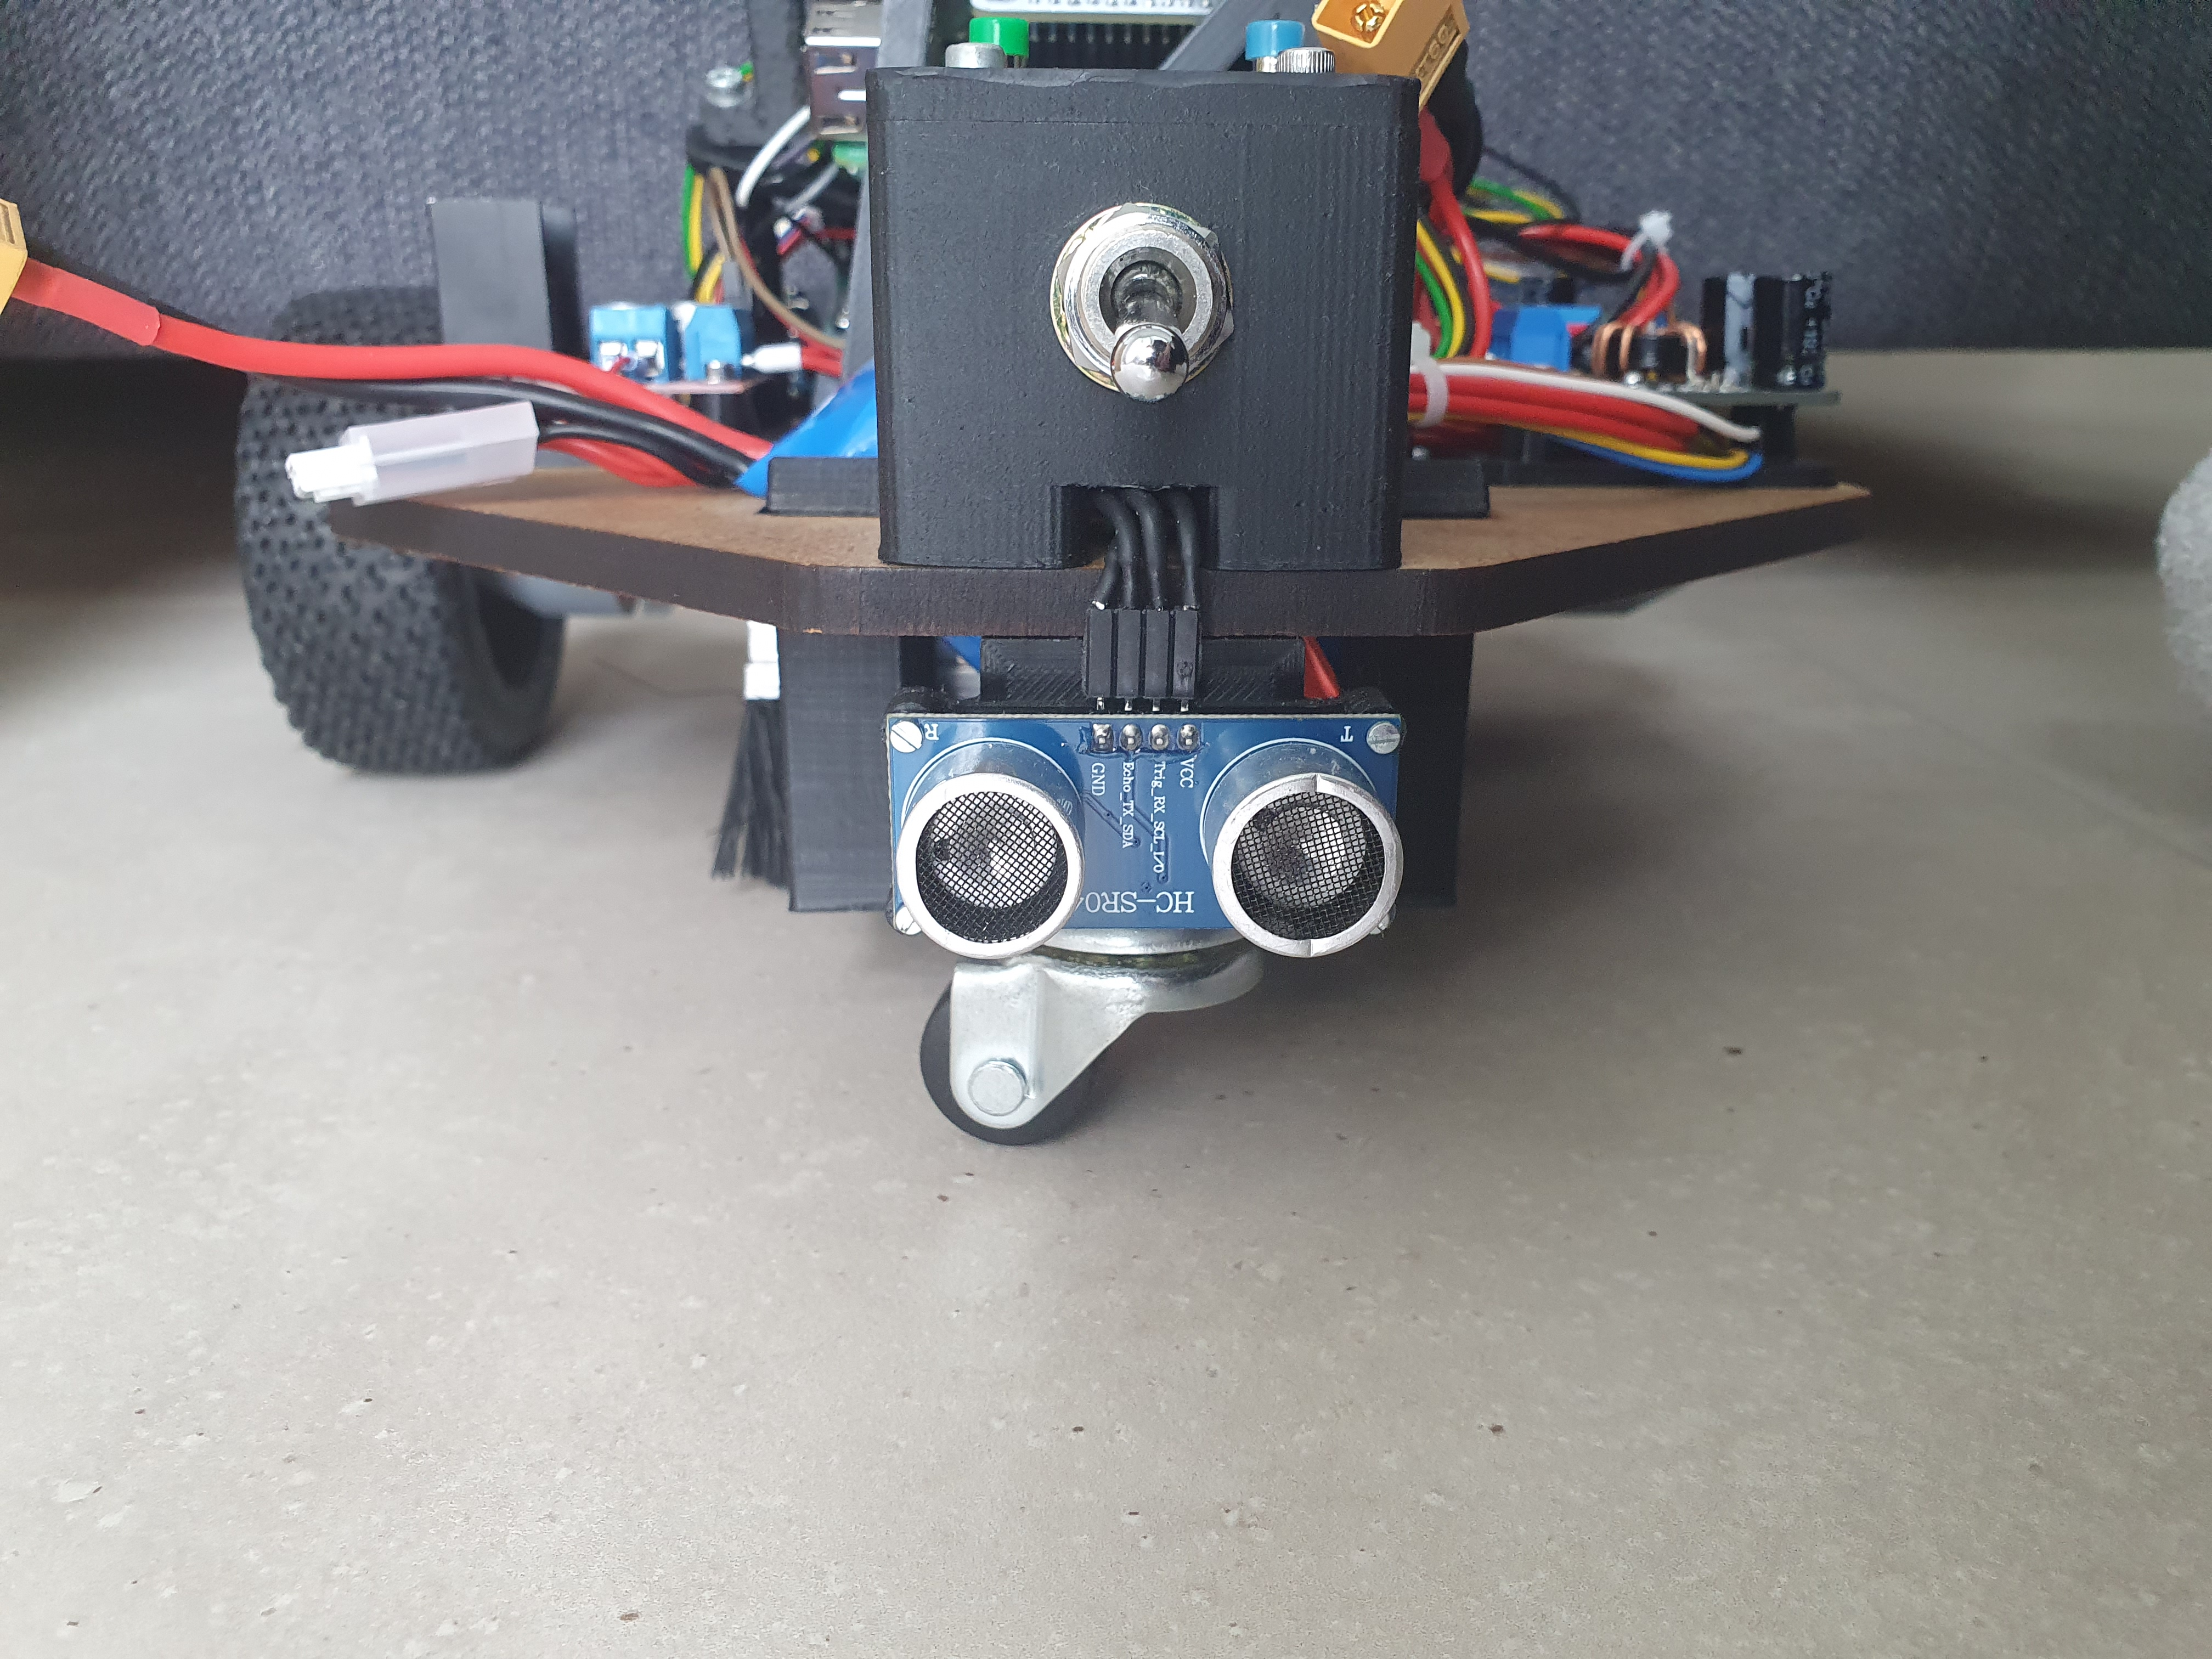
\includegraphics[width=\textwidth]{assets/ET/ultraschall/ultraschall.jpg}
  \caption{Ultraschall am Roboter}
  \label{fig:ultraschall-robi}
\end{minipage}
\hspace{0.05\textwidth} % Abstand zwischen den Bildern
\begin{minipage}[b]{0.45\textwidth}
  \centering
  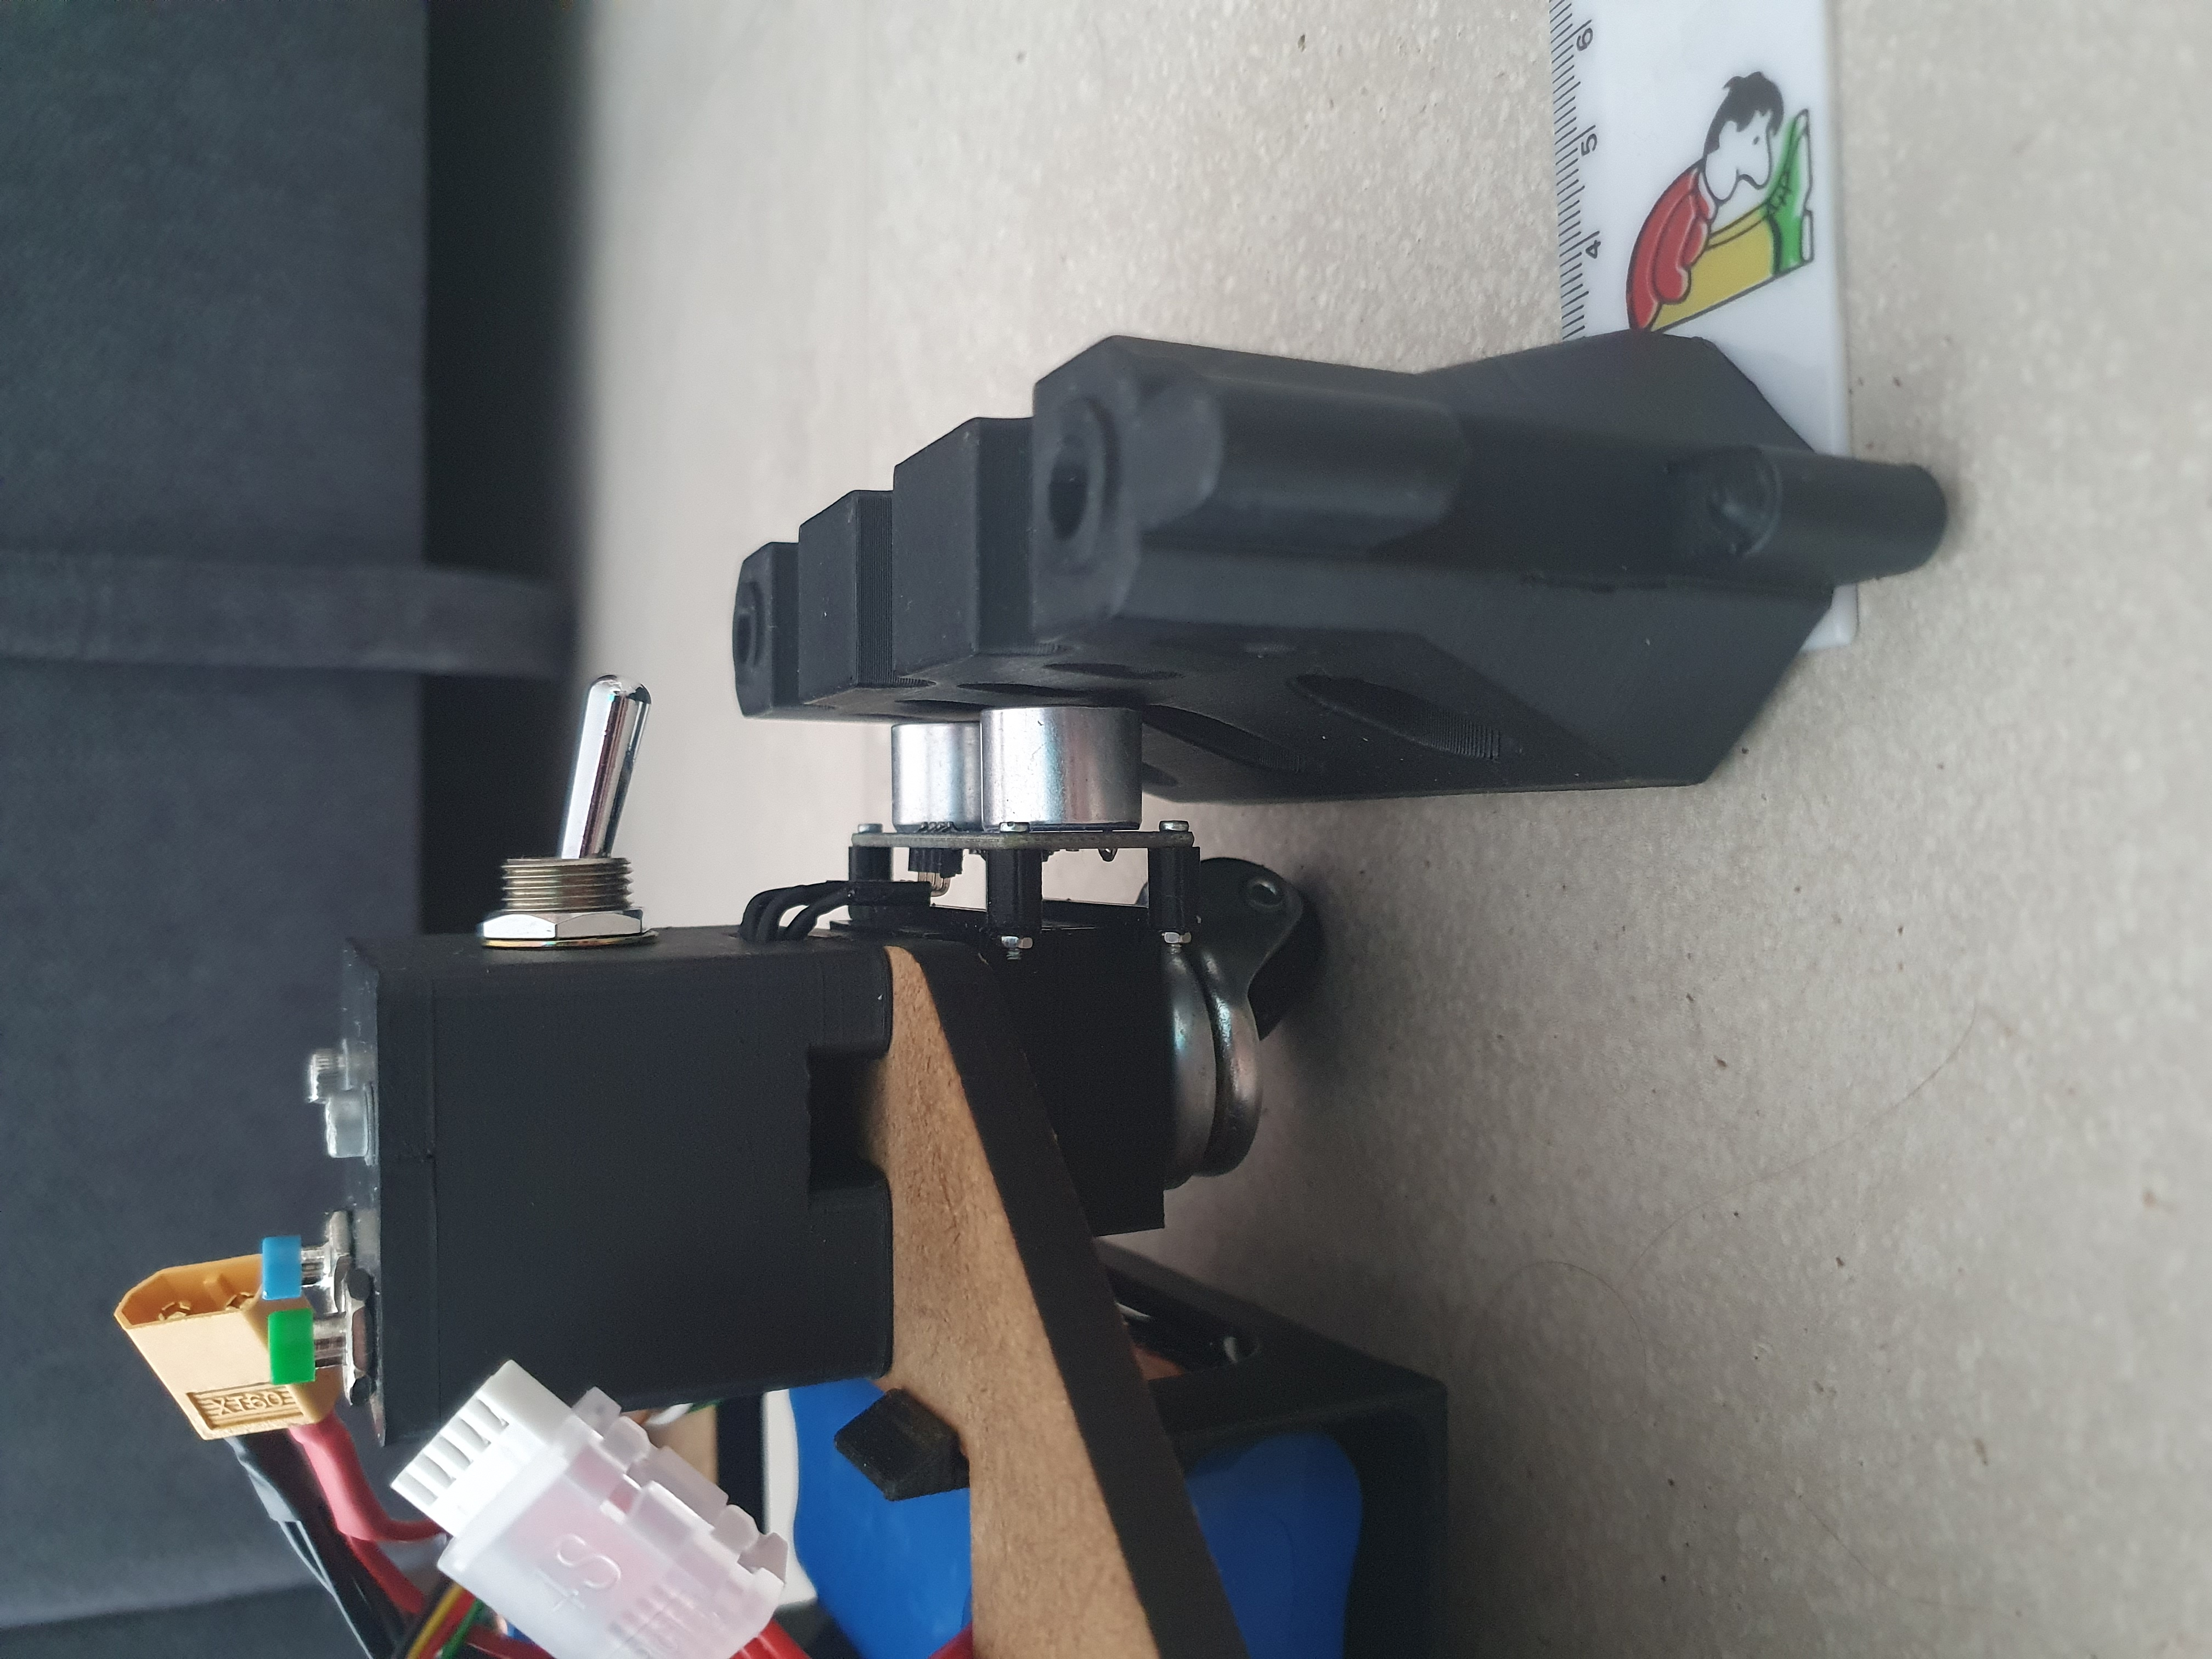
\includegraphics[width=\textwidth, angle=-90]{assets/ET/ultraschall/ultraschall-side.jpg}
  \caption{Ultraschall Höhe}
  \label{fig:ultraschall-hoehe}
\end{minipage}
\end{figure}

Der Ultraschall wurde getestet, indem die Barriere auf einem Massstab verschoben wurde. So konnten die ausgegebenen Werte mit den Werten, die auf dem Massstab ersichtlich waren, verglichen werden. Objekte können auf \pm 1cm exact erkannt werden.

\begin{figure}[H]
    \centering
    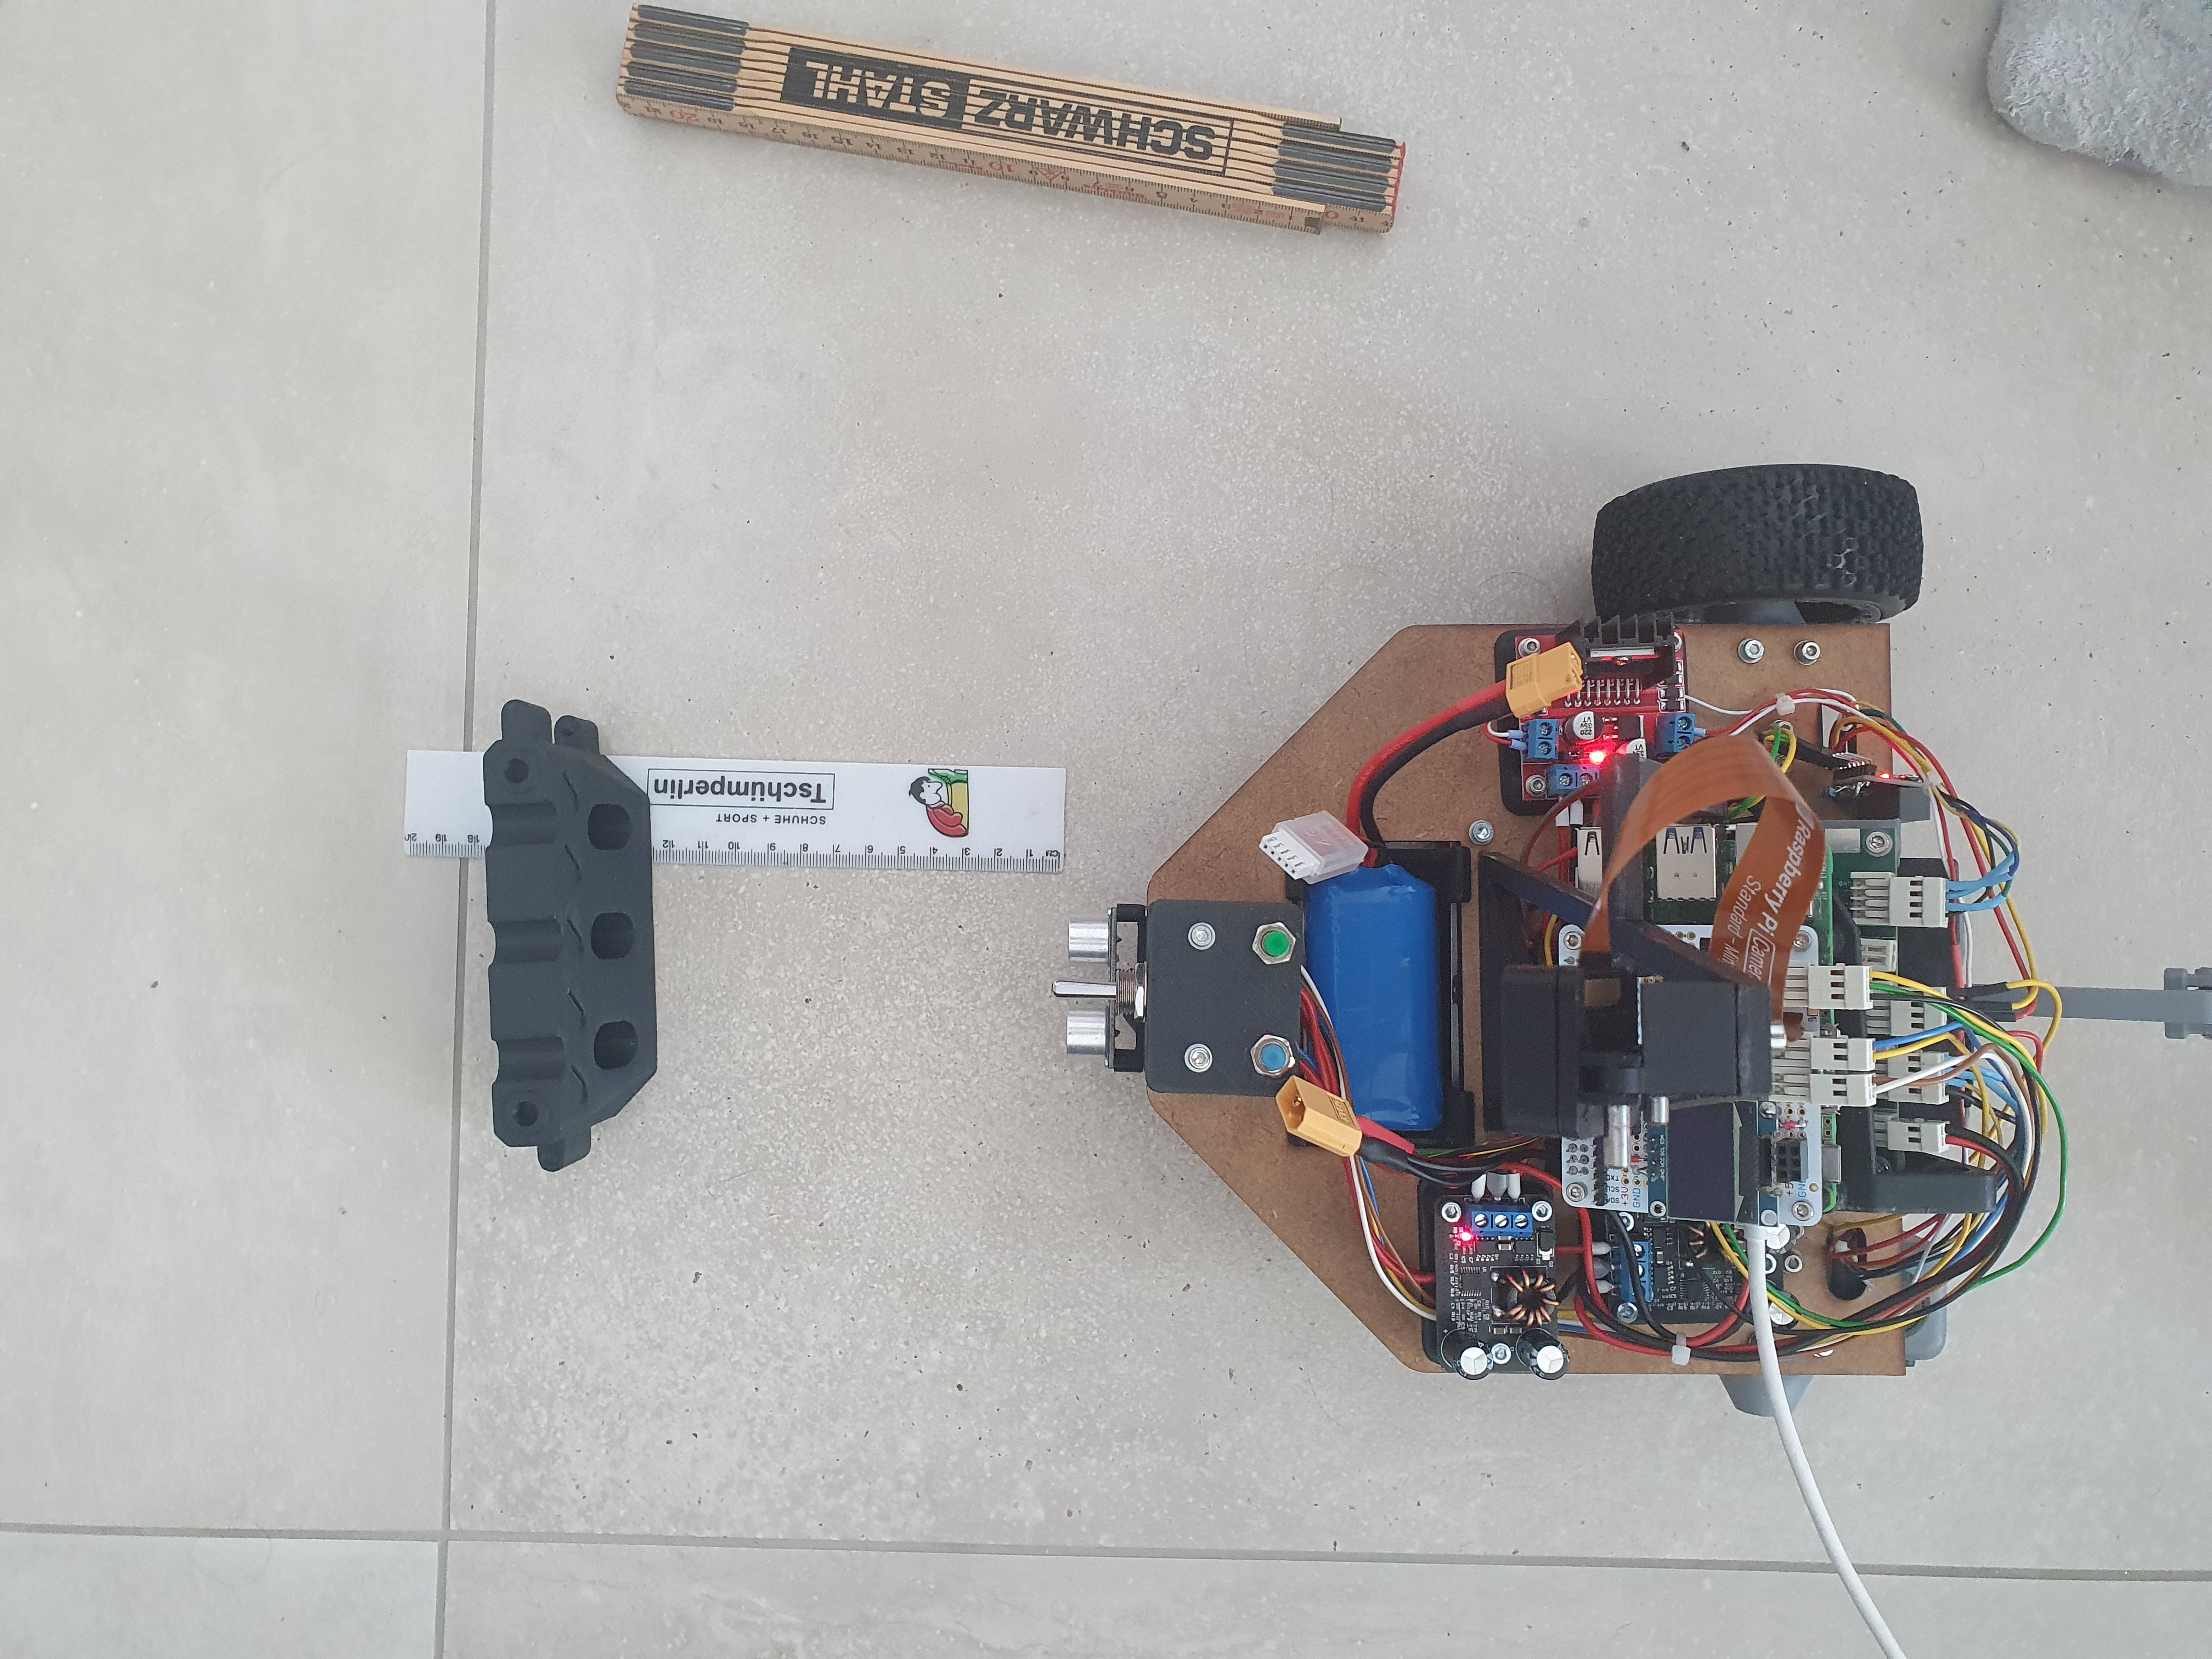
\includegraphics[width=0.5\linewidth]{assets/ET/ultraschall/ultraschall-test.jpg}
    \caption{Ultraschall Testaufbau}
    \label{fig:ultraschall-tests}
\end{figure}

\subsubsection{Kamerahalterung}
\label{Kamera Halter}

Der Winkel und die Höhe der Kamera wurden in \acrshort{pren1} an dem Testaufbau in Abbildung \ref{fig:Testaufbau zum Festlegen des Kamerawinkels} getestet. Am Testaufbau konnte der Winkel zwischen der Kamera und der Vertikalen mit Hilfe einer Schraube verstellt werden. Der Winkel wurde so gewählt, dass er für die Bildverarbeitung ideal ist. 

\begin{figure}[H]
\centering
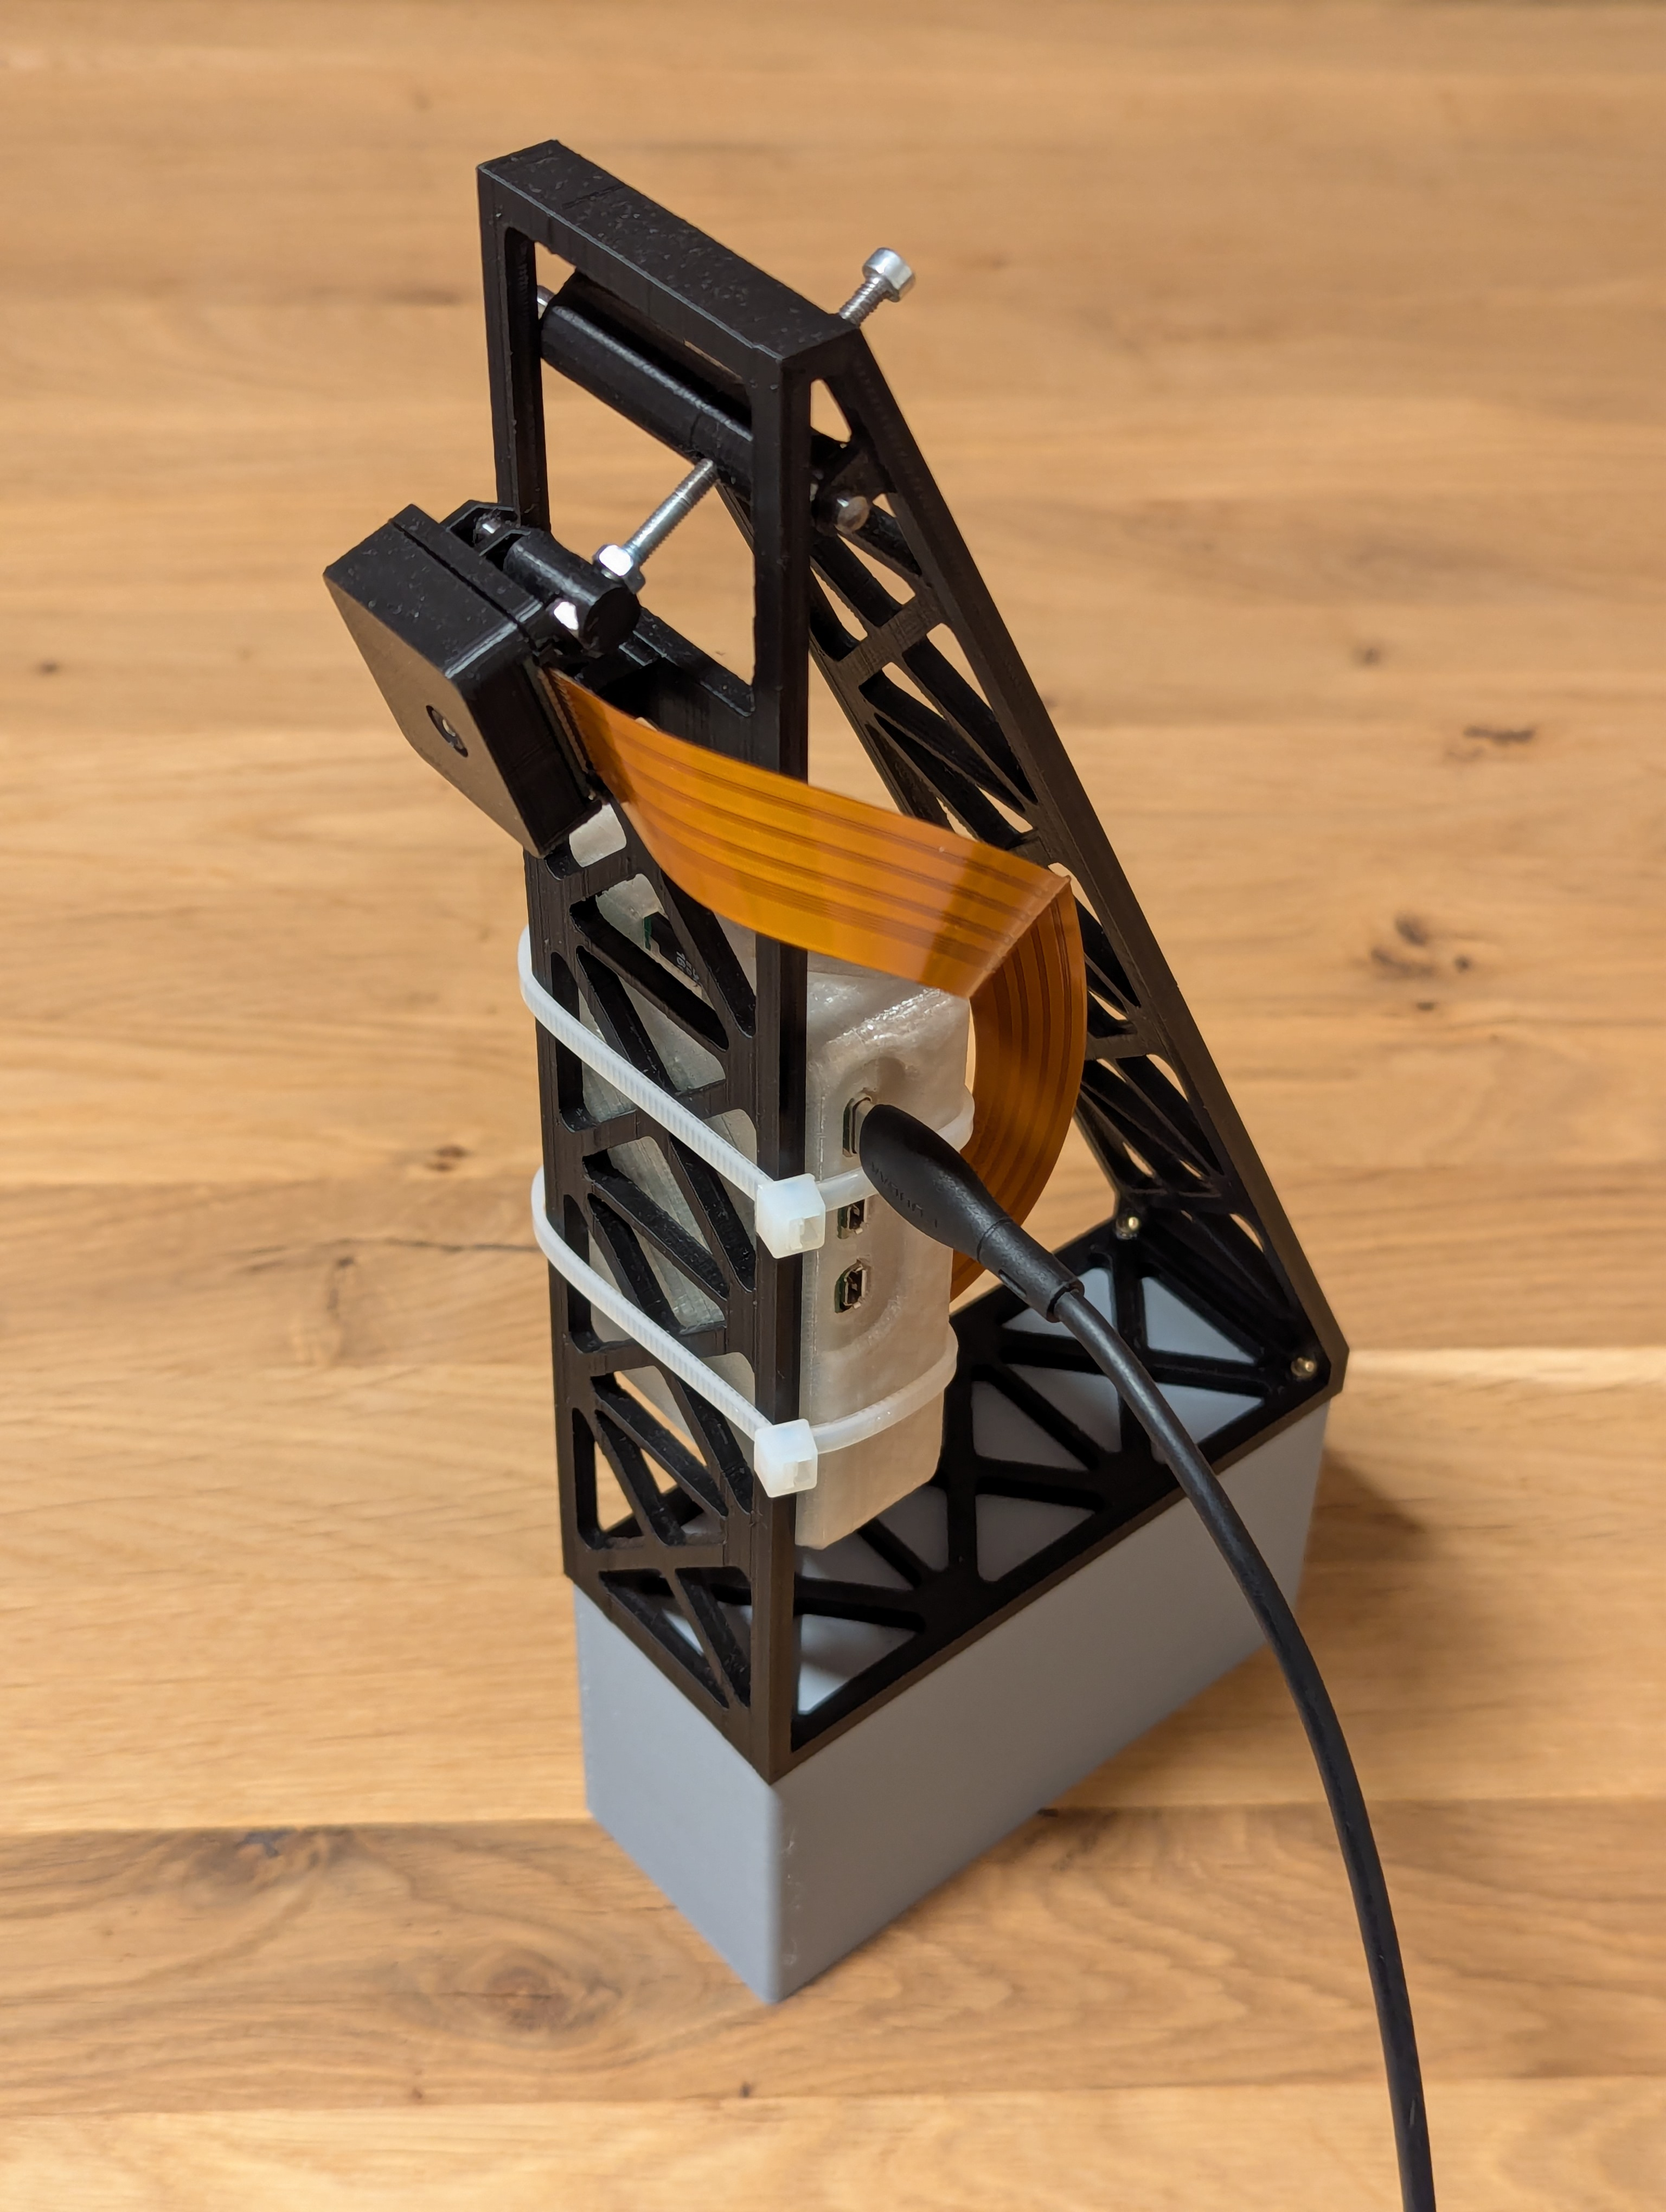
\includegraphics[width=5cm]{assets/MT/camer_tower_2.png}
\caption{Testaufbau zum Festlegen des Kamerawinkels}
\label{fig:Testaufbau zum Festlegen des Kamerawinkels}
\end{figure}


Bei der Konstruktion der Kamerabefestigung wurde darauf geachtet, dass der Winkel wie im Testaufbau gemessen 23\textdegree\ beträgt. Ebenfalls wichtig ist, dass die Linsenhöhe 242mm über dem Boden beträgt. 

 \begin{figure}[H]
\centering
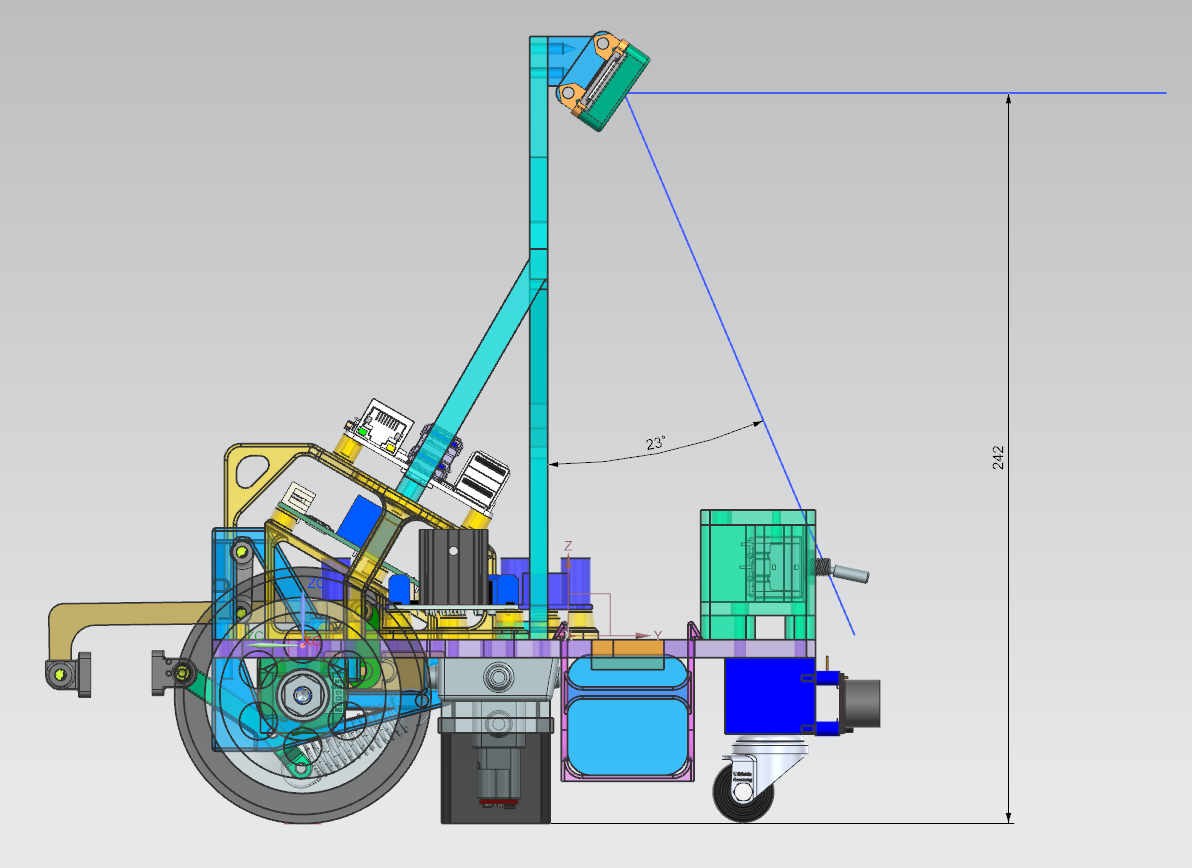
\includegraphics[width= \textwidth ]{assets/MT/Sichtfeld_Roboter.png}
\caption{Skizze der Funktionsmasse für die Kamerabefestigung}
\label{fig:Skizze der Funktionsmasse für die Kamerabefestigung}
\end{figure}

%%%%%%%%%%%%%%%%%Epic 1%%%%%%%%%%%%%%%%%%%%%%%%%%%%%%%%%%%%%%%%%%%%%%%%%%%%%%%
\subsection{Fortbewegung mit geregelter Geschwindigkeit}

\subsubsection{Print Circuit Board Design}
\label{pcb}

Um eine zuverlässige Kontaktierung der einzelnen Komponenten sicherzustellen, wird im Rahmen von \acrshort{pren2} ein Verbindungs-PCB, ersichtlich auf Abbildung \ref{fig: Verteiler PCB}, entwickelt. Dieses \acrshort{pcb} übernimmt das Management der
Spannungsversorgung für den Raspberry Pi und den \gls{tinyk22}. Zudem werden sämtliche Signale,
die vom \gls{tinyk22} erfasst und verarbeitet werden sollen, entsprechend verbunden.

\begin{figure}[H]
\centering
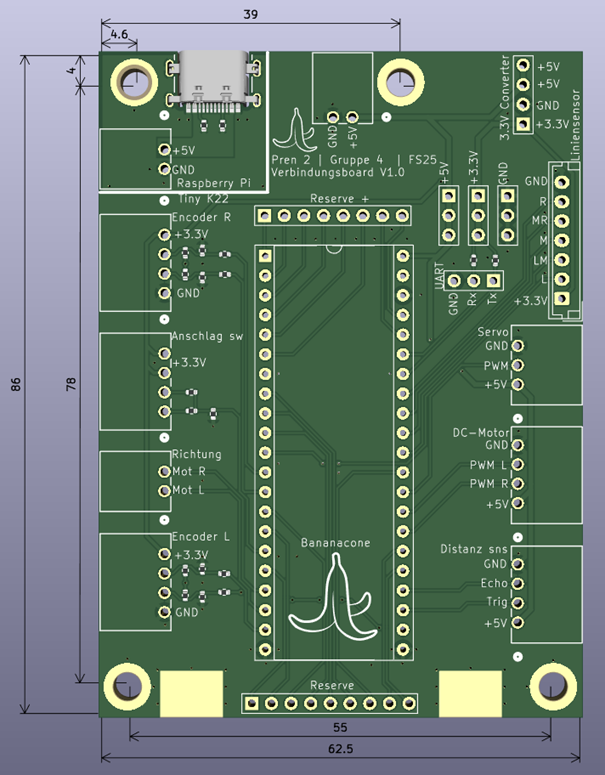
\includegraphics[width=5cm, height=6cm]{assets/ET/PCB/VerteilerPCB_unbestueckt.png}
\caption{Verteiler PCB}
\label{fig: Verteiler PCB}
\end{figure}

Von dem PCB wurden fünf Exemplare bestellt. Ebenso sind von dem \gls{tinyk22} mehrere Exemplare vorhanden. Das PCB zusammen mit dem \gls{tinyk22} ist auf Grafik \ref{fig: Verteiler PCBA} gezeigt. Somit ist das Risiko der kaputten Elektroteile nicht mehr relevant.

\begin{figure}[H]
\centering
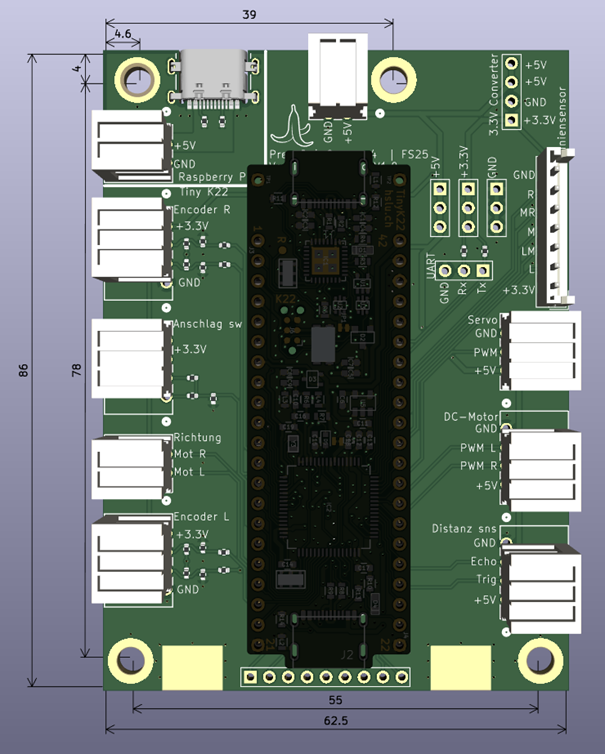
\includegraphics[width=5cm, height=6cm]{assets/ET/PCB/VerteilerPCB_bestueckt.png}
\caption{Verteiler PCBA}
\label{fig: Verteiler PCBA}
\end{figure}

TODO nachfolgende Linie korrekt? Oder Ausversehen eingefügt wroden?\\
\gls{pren2}



\subsubsection{Pinout und Softwaregrundlagen}

TODO: Die vier Bilder gehören zusammen (Formatierung)

Als Grundlage für die Software diente das Projekt aus dem Modul \textit{Microcontroller Fundamentals}. Dieses enthielt ein solides Gerüst, das im Verlauf angepasst wurde. Dabei wurden verschiedene Codeabschnitte ergänzt, überarbeitet oder entfernt. Als Entwicklungsumgebung kam \textit{MCUXpresso} zum Einsatz.

Die Initialisierung der Pins erfolgte auf Basis der Belegungen aus Abbildung~\ref{fig:Pinout TinyK22} und Abbildung~\ref{fig:Pinout Raspy Hat}. Im Vergleich zur ursprünglichen Planung in \gls{pren1} (siehe Abbildung~\ref{fig:Pinout PREN 1}) hat sich das finale Pinout bis zum Ende von \gls{pren2} (siehe Abbildung~\ref{fig:Pinout PREN 2}) in mehreren Punkten verändert.

Drei ursprünglich für die Liniensensoren vorgesehene Pins mussten aufgrund der verwendeten Sensorbank entfallen. Der Buzzer sowie der Startknopf wurden auf das Raspberry-HAT verlagert. Zudem wurde die Richtungsauswahl von zwei auf vier Pins erweitert, um eine differenziertere Steuerung zu ermöglichen. Zusätzlich wurde eine $I^2C$-Schnittstelle implementiert, um weitere Sensoren anbinden zu können.


\begin{figure}[H]
\centering
\begin{minipage}[b]{0.45\textwidth}
  \centering
  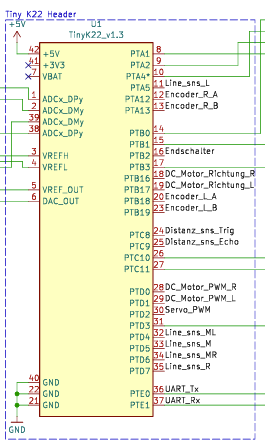
\includegraphics[width=\textwidth]{assets/ET/Software/Tiny_Pinout.png}
  \caption{Pinout Tiny K22}
  \label{fig:Pinout TinyK22}
\end{minipage}
\hspace{0.05\textwidth} % Abstand zwischen den Bildern
\begin{minipage}[b]{0.45\textwidth}
  \centering
  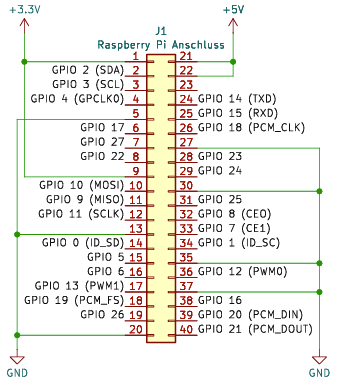
\includegraphics[width=\textwidth]{assets/ET/Software/RaspyHat_Pinout.png}
  \caption{Pinout Raspberry Pi}
  \label{fig:Pinout Raspy Hat}
\end{minipage}
\end{figure}


\begin{figure}[H]
\centering
\begin{minipage}[b]{0.45\textwidth}
  \centering
  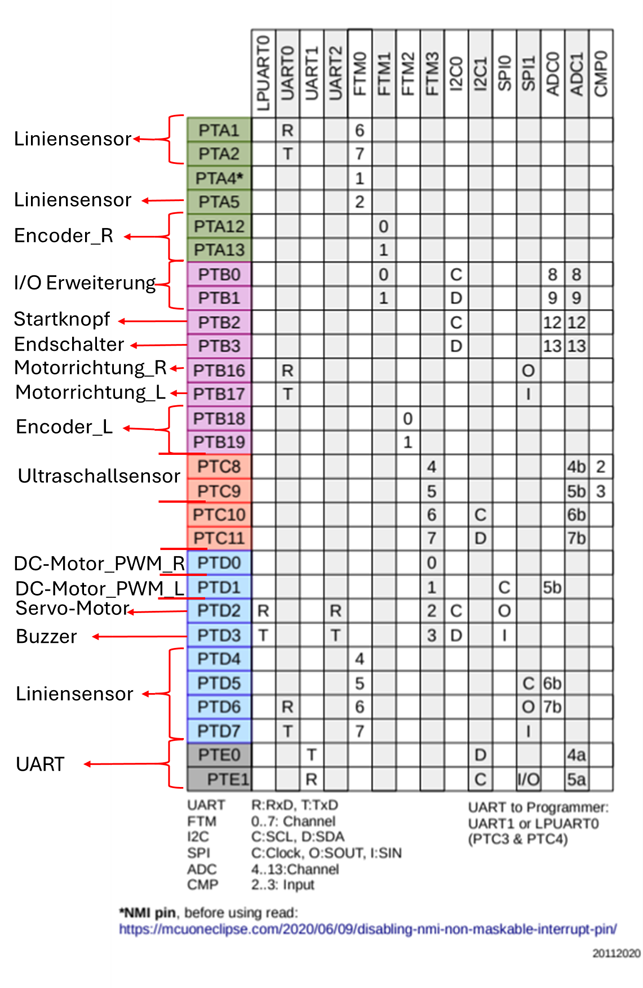
\includegraphics[width=\textwidth]{assets/ET/PINOUT/Pinout_PREN1.png}
  \caption{Pinout PREN 1}
  \label{fig:Pinout PREN 1}
\end{minipage}
\hspace{0.05\textwidth} % Abstand zwischen den Bildern
\begin{minipage}[b]{0.45\textwidth}
  \centering
  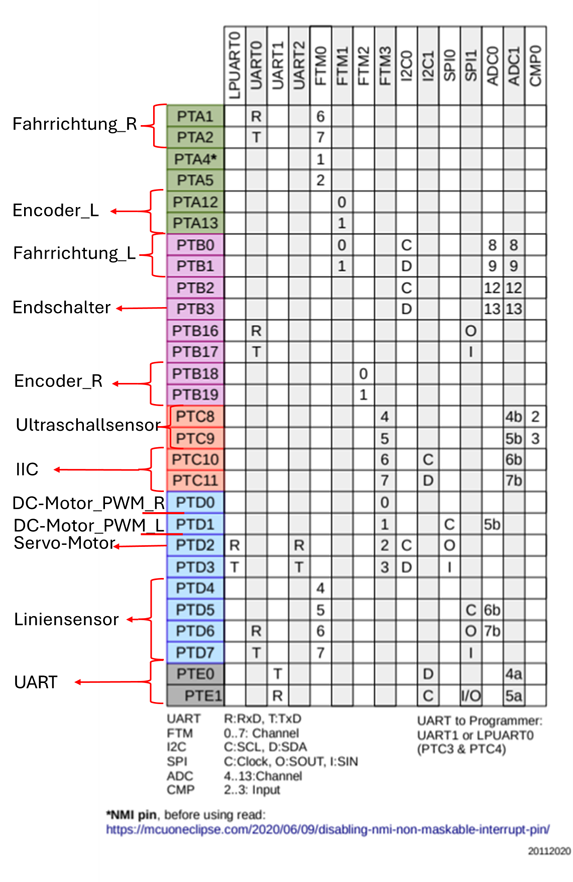
\includegraphics[width=\textwidth]{assets/ET/PINOUT/Pinout_PREN2.png}
  \caption{Pinout PREN 2}
  \label{fig:Pinout PREN 2}
\end{minipage}
\end{figure}





\subsubsection{Spannungsversorgung und Leistungsberechnung}


In der Tabelle \ref{tab:spannungsversorgung} werden alle Verbraucher aufgezeigt mit ihrer Betriebsspannung wie auch die maximale Stromaufnahme. Anhand dieser Daten konnte die Wahl eines geeigneten Akkus getroffen werden. Die Spannungsversorgung kann mittels eines Not-Aus Schalters von den Verbrauchern getrennt werden, ausser das Raspberry Pi 5 wird dabei als einziger Verbraucher nicht Stromlos gemacht. Damit wird die Möglichkeit von Datenkorruption auf der SD-Karte verringert. Berechnet man von jedem Verbraucher die Leistung kommt man auf eine maximale Gesamtleistung von 101W. Der vorgesehene Akku, hat eine Spannung von 14.8V und eine Kapazität von 3000mAh. Unter maximaler Leistung könnte der Roboter für ca. 25 Minuten Funktionieren \ref{eq:Energieverbrauch}.

\begin{equation}
    t = \frac{E}{P} = \frac{U \cdot Q}{P} = \frac{14{,}8\,\text{V} \cdot 10800\,\text{As}}{105\,\text{W}} \approx 1{'}520\,\text{s} = 25\,\text{Minuten} 
    \label{eq:Energieverbrauch}
\end{equation}



\newpage

\begin{table}[h!]
\centering
\renewcommand{\arraystretch}{1.3}
\begin{tabular}{@{} l c c l @{}}
\toprule
\textbf{Verbraucher}         & \textbf{Spannung} & \textbf{Strom (geschätzt)} & \textbf{Bemerkung} \\
\midrule
2x DC-Motor                  & 12V              & 6A gesamt               & Ansteuerung über Motortreiber \\

Motortreiber & 5V               &  100mA              & Logikversorgung \\

2x Encoder & 3.3V               &  150mA gesamt             &- \\

Servomotor                   & 5V               &  500mA                 & PWM-gesteuert, kurzzeitig hohe Last \\

Liniensensor         & 5V               &  150mA                  & IR-LED's und Sensoren \\

Ultraschall & 5V               &  200mA              &- \\

Raspberry Pi 5              & 5V               & 3-5A                      & über USB-C \\

Tiny K22             & 5V               & 500mA                      & - \\

\bottomrule
\end{tabular}
\caption{Übersicht der Spannungsversorgung des Roboters}
\label{tab:spannungsversorgung}
\end{table}



\subsubsection{Motoren ansteuern und auslesen}
\label{motoren-encoder}


Nachdem die erste Ausführung der Software für die Motoren mit den beiden Encodern vorhanden war, wurde der implementierte Code mithilfe eines provisorischen Aufbaus getestet. Unter einem provisorischen Aufbau versteht man die Verwendung eines Breadboards mit dem \gls{tinyk22} und einem Speisegerät. Dies ist auf Abbildung \ref{fig: Motorentest} ersichtlich.

\begin{figure}[H]
\centering
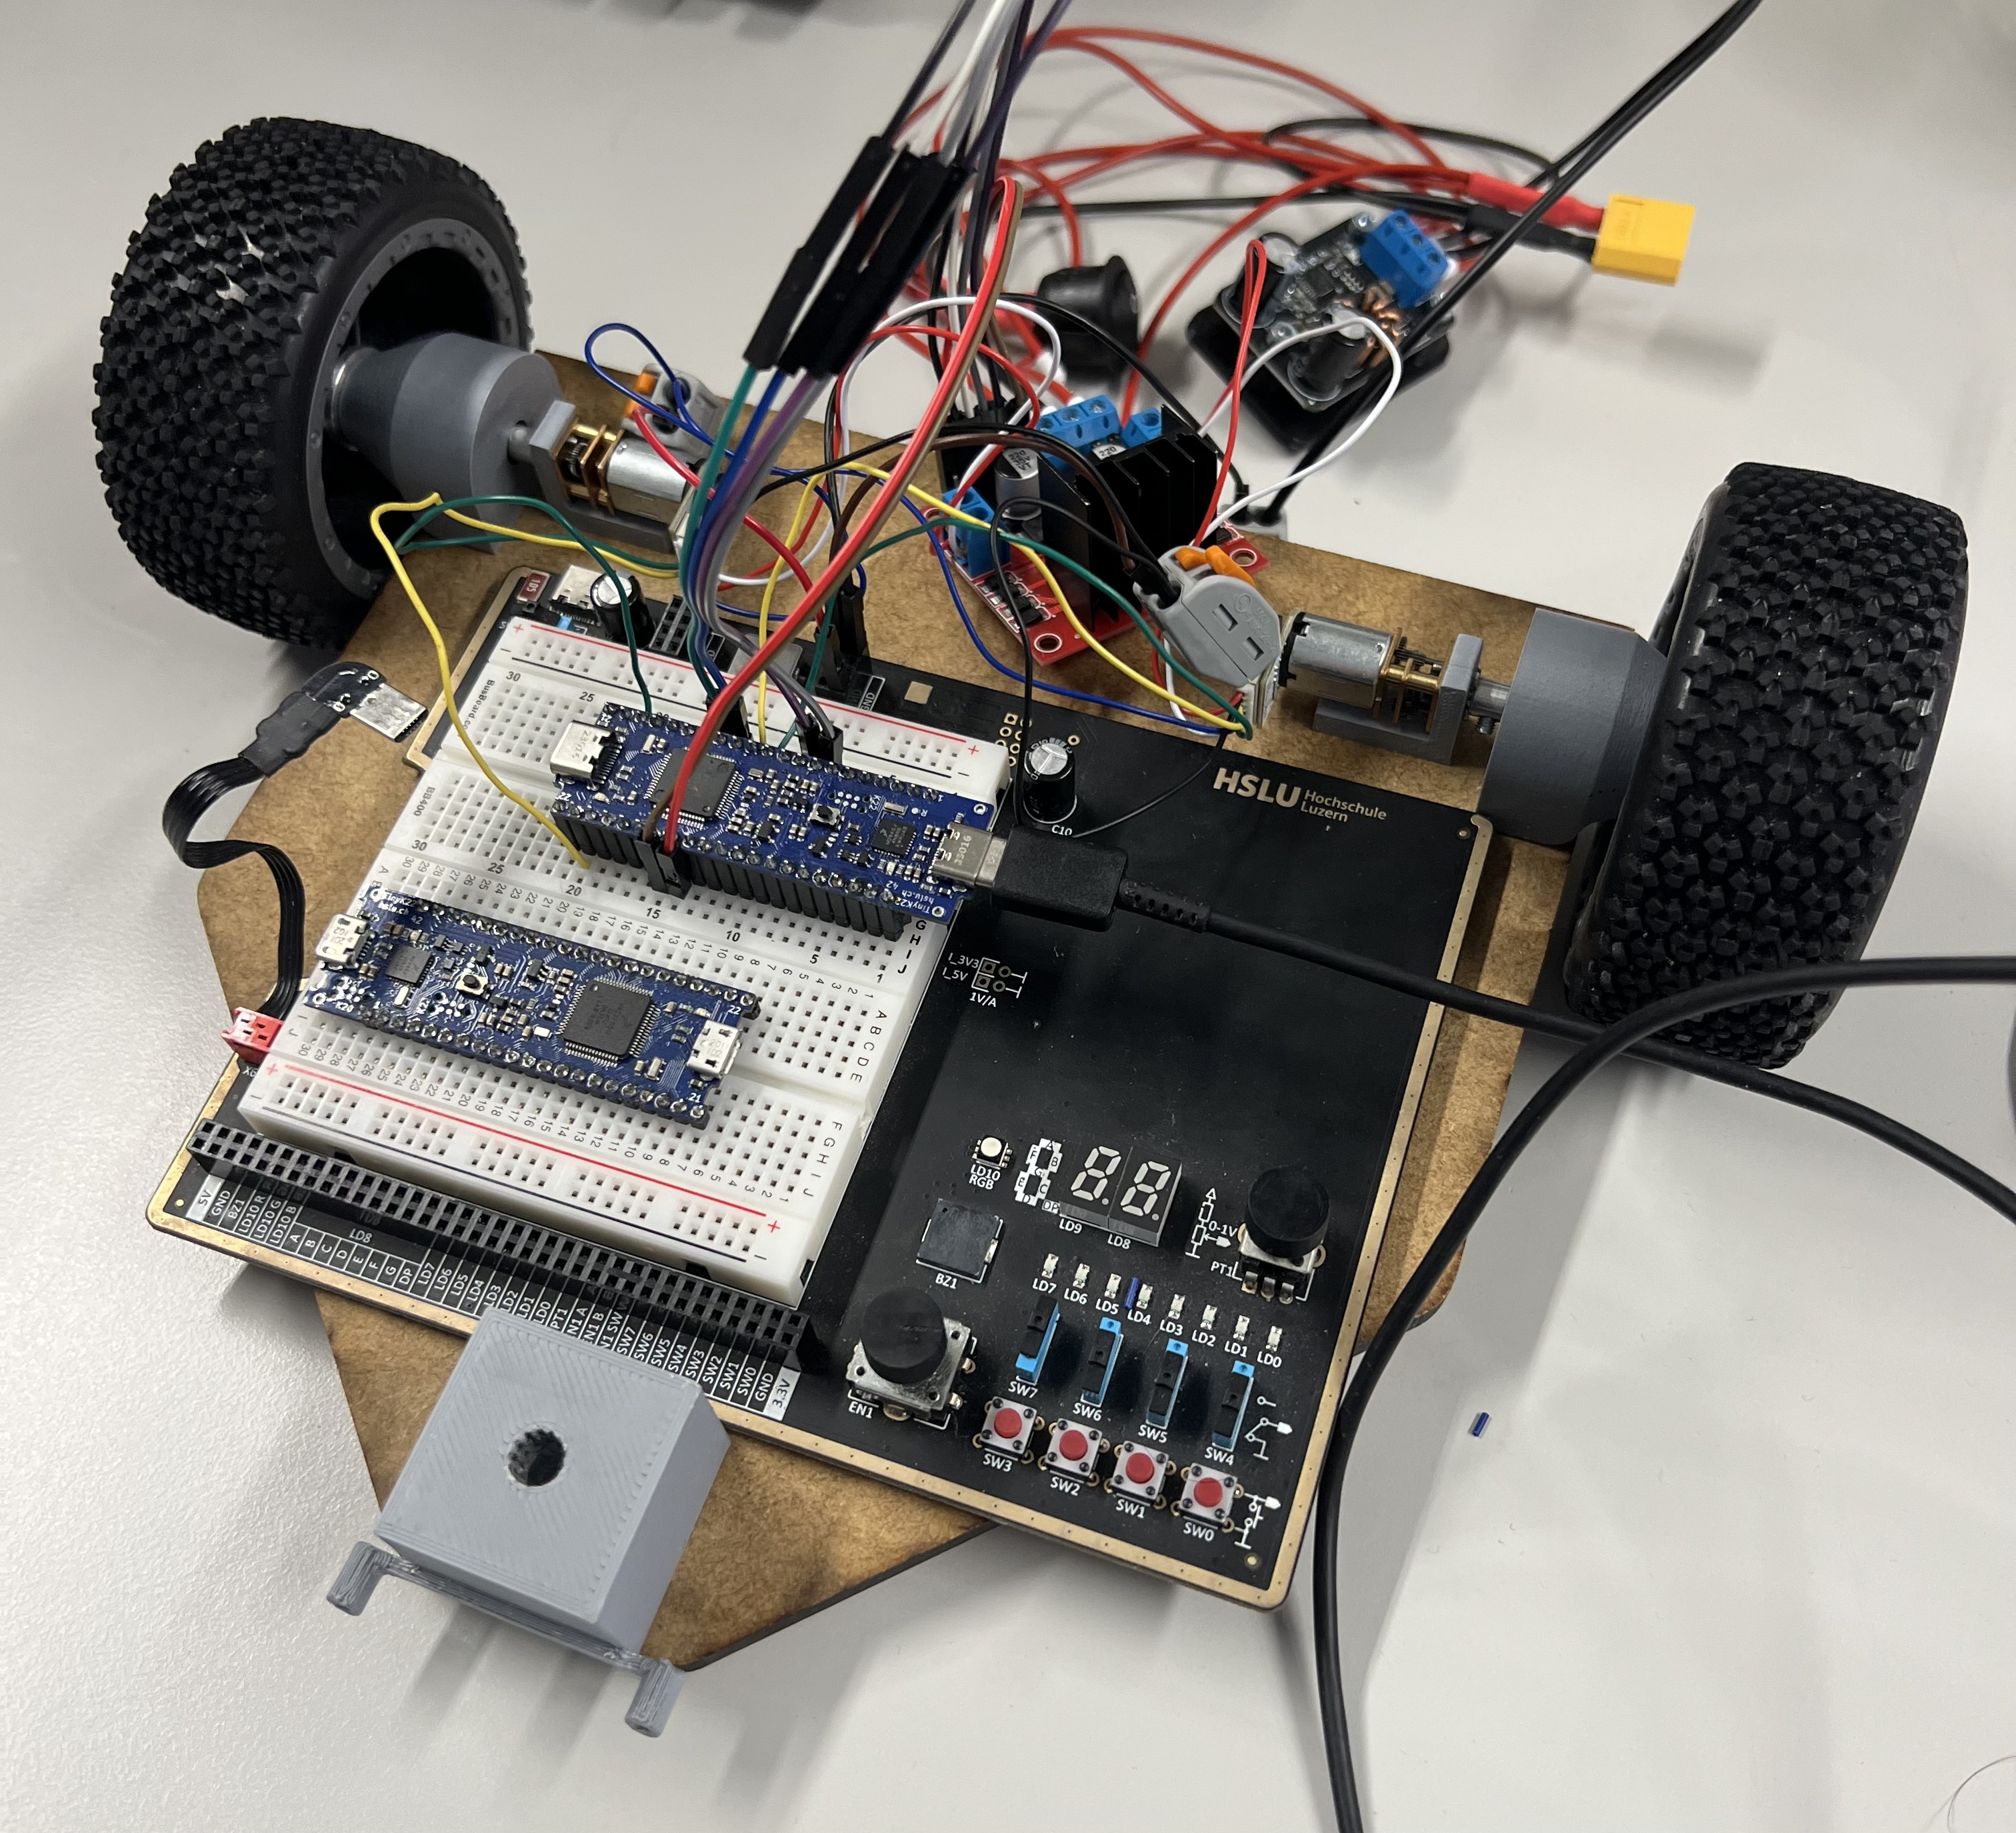
\includegraphics[width=10cm, height=8cm]{assets/ET/Motoren/Motorentest.jpeg}
\caption{Motorentest}
\label{fig: Motorentest}
\end{figure}


Allerdings kam bereits der Motortreiber zum Einsatz, der auch im späteren Endprodukt verbaut werden soll. Nach anfänglichen Schwierigkeiten bei der Initialisierung des Quadratur-Encoder-Modus auf dem \gls{tinyk22} konnten die ersten Meter erfolgreich zurückgelegt werden. Der zugrunde liegende Fahralgorithmus basiert darauf, die Werte beider Encoder zu mitteln, um die gefahrene Strecke zu ermitteln (siehe Gleichung~\ref{eq:gefahren}).

\begin{equation}
    gefahrenMEAN_{cm} = \frac{gefahrenR_{cm} + gefahrenL_{cm}} {2} 
    \label{eq:gefahren}
\end{equation}

Mit den ersten Erkenntnissen aus dem Test konnte die Software weiter angepasst werden, um immer präzisere Fahrmanöver auszuführen. 




%%%%%%%%%%%%%%%%%Epic 2%%%%%%%%%%%%%%%%%%%%%%%%%%%%%%%%%%%%%%%%%%%%%%%%%%%%%%%

\subsection{Auf Linien des Graphes bewegen}
\label{Auf Linien des Graphes bewegen}

\subsubsection{Liniensensor auslesen}
\label{Liniensensor auslesen}

In einem ersten Durchlauf wurde ein Code implementiert, um die Funktion mit dem \gls{tinyk22} zu testen. Mittels eines Timers wurden die einzelnen Pins in einem genügend grossen Zeitabstand von \acrfull{vcc} auf Input Capture umgeschaltet. Nach dem Umschalten auf Input Capture, sollten sich die Kondensatoren je nach Reflektion des Untergrundes in unterschiedlichen Zeiten laden. Dieses Verhalten konnte im Testprogramm dann auch erfolgreich festgestellt werden durch die unterschiedlichen Werte im Timer Register des Input Capture Modus.


\subsubsection{Linie folgen mit PD-Regelung}
\label{Linie folgen mit PD-Regelung}

Nachdem die Auslesung des Liniensensors erfolgreich getestet wurde, konnte die eigentliche Linienregelung implementiert werden, wovon ein Ausschnitt auf Abbildung \ref{fig:Ausschnitt der Implementation der PD-Regelung} ersichtlich ist. Damit möglichst dynamisch und mit möglichst wenig Schwingungen gefahren werden kann, wurde ein PD-Regler ausgewählt. Bei jedem Neustart des Roboters, liest eine Kalibrierungsfunktion die Soll-Werte der einzelnen Sensoren ein. Beim Kalibrieren muss der Roboter immer in seiner Soll-Fahrposition stehen. Die periodisch aufgerufene Reglerfunktion berechnet dann aus dem Soll-Wert und dem aktuellen Sensorwert (Ist-Wert) die Abweichung. Diese Fehler werden zu einem Gesamtfehler mit einer Gewichtung der Sensoren von aussen nach innen zunehmend berechnet. Dieser Gesamtfehler wird dann mit dem P- und D-Anteil zu einem Korrekturwert weiter verrechnet. Der Proportionalanteil (P) sorgt dafür, dass das Fahrzeug bei einem grösseren Fehler stärker korrigiert, während der Differentialanteil (D) auf schnelle Änderungen des Fehlers reagiert und so Schwingungen dämpft. Der Korrekturwert wird dann genutzt um die beiden \acrfull{pwm} Signale der Motoren zu senken oder erhöhen, je nach Abweichung zur Linie.

 \begin{figure}[H]
\centering
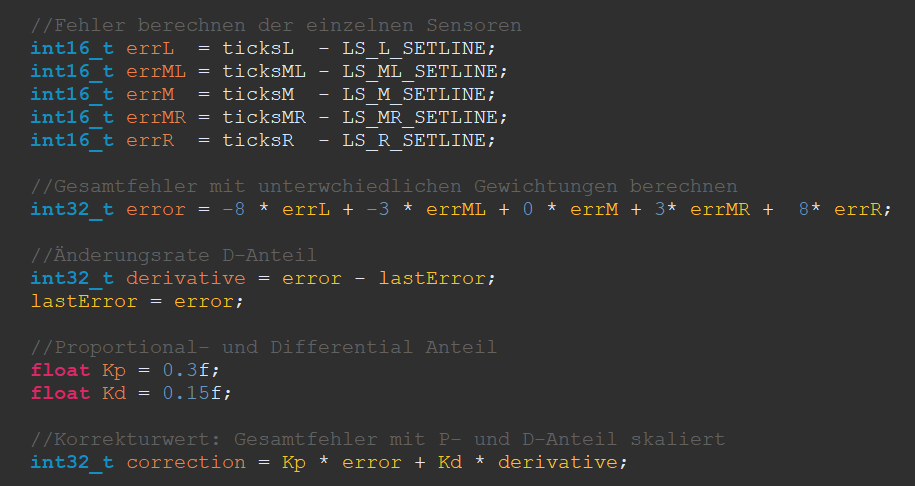
\includegraphics[width= \textwidth ]{assets/ET/PD-Regler/PD-Regler_Code_Pren2.png}
\caption{Ausschnitt der Implementation der PD-Regelung}
\label{fig:Ausschnitt der Implementation der PD-Regelung}
\end{figure}


\subsubsection{Liniensensor mit Abschirmung anbringen}

Nach dem ersten Test wurde der Liniensensor am Fahrzeug mit der Abschirmung angebracht (siehe Abbildung \ref{fig:enter-label}). Dank diesem Aufbau konnte mit der weiteren Implementierung fortgefahren werden. Für die Feineinstellung wurden die einzelnen Sensorwerte auf dem Originalboden und dem Klebeband ausgemessen, da dies essenziell ist, um die Regelung sauber abzustimmen.


\begin{figure}[H]
    \centering
    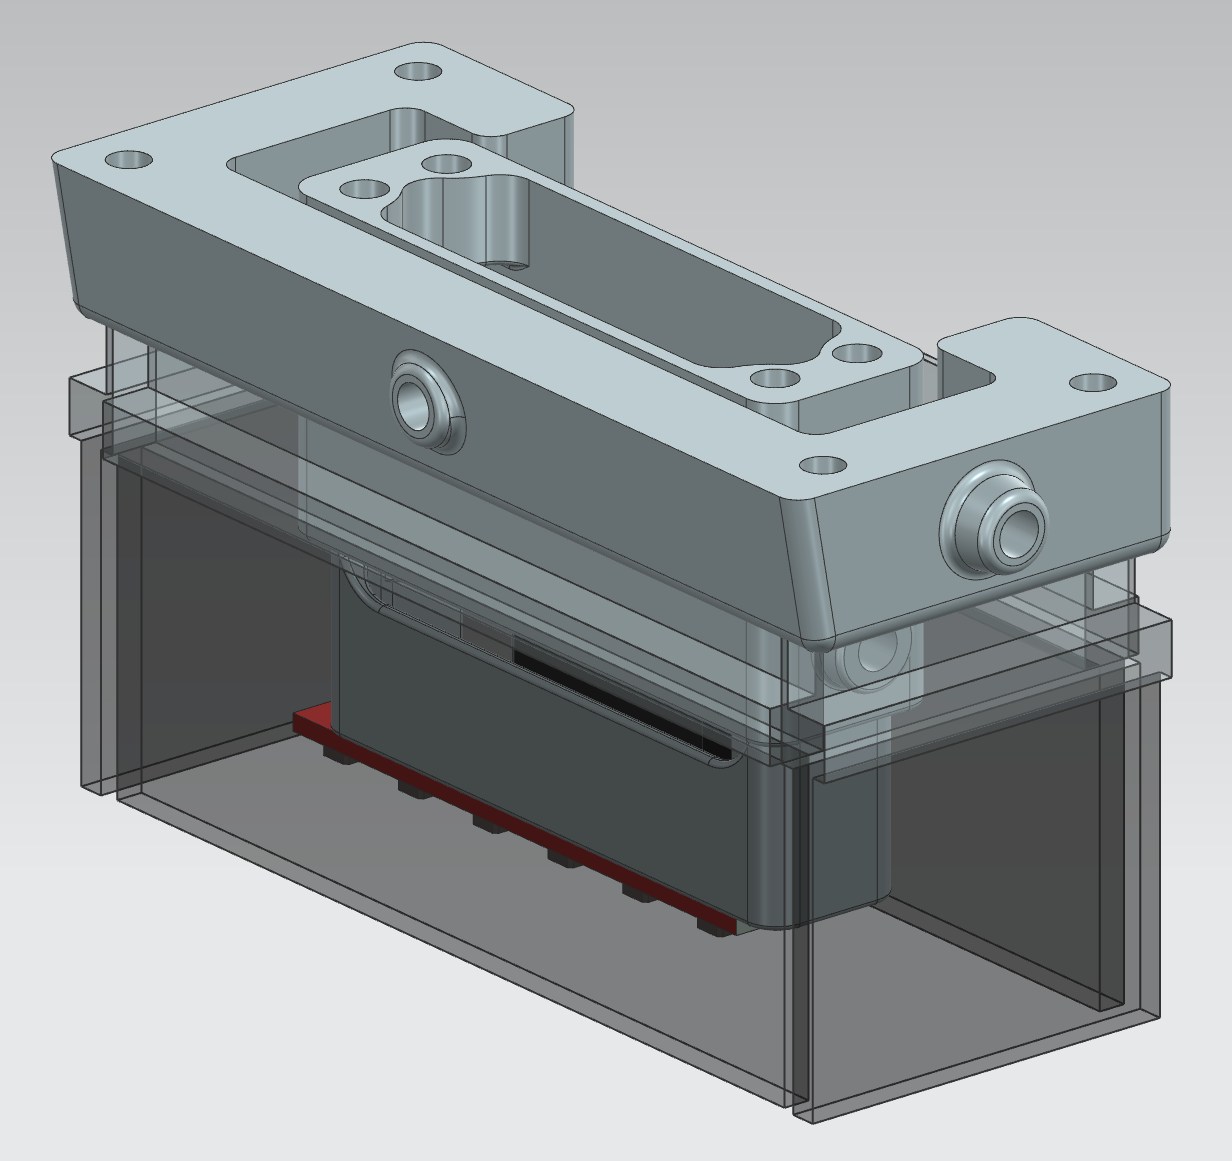
\includegraphics[width=0.5\linewidth]{Sensor montiert.png}
    \caption{Sensor montiert}
    \label{fig:enter-label}
\end{figure}


\newpage
%%%%%%%%%%%%%%%%%Epic 3%%%%%%%%%%%%%%%%%%%%%%%%%%%%%%%%%%%%%%%%%%%%%%%%%%%%%%%

\subsection{Bis zum nächsten Knoten fahren}

\subsubsection{Liniensensor}

Die Liniensensoren wurden wie geplant implementiert. Durch das Ummuxen der Pins von GPIO-Output (High) auf den Input Capture Modus, wird die Ladezeit eines Kondensators gemessen. Diese Zeit (ausgedrückt in Ticks) liefert Informationen darüber, ob sich das Fahrzeug über dem Soll-Fahrweg befindet oder davon abweicht. Während der Fahrt werden die Sensor-Pins periodisch zwischen GPIO High und Input Capture umgeschaltet, um kontinuierlich neue Messwerte zu erhalten. Die erfassten Ticks werden in einer PD-Regelung weiter verarbeitet, welche die Abweichung zur Soll-Position (Linie) berechnet und entsprechend die Motoren nachsteuert. Diese Regelung ergänzt die Wegmessung über die Encodersensoren und erhöht die Spurtreue, indem sie sicherstellt, dass das Fahrzeug die Linie nicht verlässt. Das Erkennen ob der Roboter auf einem Wegpunkt steht oder nicht, wird ebenfalls mittels der Sensorenwerte geprüft. Da beim erreichen des Wegpunktes im Optimalfall alle Sensoren auf der weissen Oberfläche stehen, weichen die Werte der aktuellen Ticks stark der Sollwerte ab. Somit kann ein Wegpunkt klar identifiziert werden und der Roboter kann anhalten.



